\chapter{Experimental results}
\label{chap:outcome}
\setheader{Experimental outcome}
In this chapter, the final results will be presented first (a few results can be found on page \pageref{fig:res_NX506_pluis} to \pageref{fig:res_NX501_pluis}).
Thereafter the results are discussed: are there notable results, which do or do not match with the expectations (Section \ref{sec:ms-expectations}).
A little conclusion will be provided at the end of this chapter.

\section{Results}
\label{sec:results}
After measuring, processing and equalizing, some of the results are presented at the end of this chapter (from page \pageref{fig:res_NX506_pluis} to \pageref{fig:res_NX501_pluis}).
For there are conducted a lot of measurements, only a handful of result is displayed in this thesis for comparison.
For more results, the writers can be contacted.

The results that will be discussed are from four different measurement set-ups:
\begin{itemize}
\item \nexus, labelled with number six in mid-air, for a full sphere (Figure \ref{fig:res_NX506_pluis});
\item \nexus, labelled with number six face up on the surface, for a sphere with $\phi\in[0,135]^\circ$ (Figure \ref{fig:res_NX506_FU});
\item \nexus, labelled with number six face down on the surface, for a sphere with $\phi\in[0,135]^\circ$ (Figure \ref{fig:res_NX506_FD}); and,
\item \nexus, labelled with number one in mid-air, due to time constrains only measured for a sphere with $\phi\in[0,90]^\circ$ (Figure \ref{fig:res_NX501_pluis}).
\end{itemize}

There are a few things to notice from these given results.
When the smartphone microphone is turned away from the loudspeaker, the gain is less then when the smartphone microphone is turned toward the loudspeaker (Figure \ref{fig:res_NX506_pluis_90}).
For elevations higher or smaller than $90^\circ$, this effect is less (Figure \ref{fig:res_NX506_pluis_42}, \ref{fig:res_NX506_pluis_138}).

%Effect of surface
The addition of the surfaces changes the reception of the signals, especially the signals from below the surface (Figure \ref{fig:res_NX506_FU_135}, \ref{fig:res_NX506_FD_135}).

%Difference between two phones
Between the two phones there is a visible difference between the behaviour of the directivity (Figure \ref{fig:res_NX501_pluis}), the gain of the the phone labelled with number one seems higher than the gain of the phone labelled with number six.
In the next section, these results will be placed in different perspectives.
\clearpage
\section{Discussion}
\label{sec:discussion}

In this chapter, the data will be looked at and compared.
This will be mostly done by the Figures from page \pageref{fig:res_NX506_pluis} to page \pageref{fig:res_NX501_pluis}.
One of the first things that stands out is that the directivity is non-symmetric in the $\theta$-axis (Figure \ref{fig:res_NX506_pluis}).
This can be explained by the lack of symmetry in \nexus.
Its microphone is not positioned in the middle of the smartphone, but 2 cm to the right, which causes the non-symmetrical behaviour.

The microphone also seems to lack quality, comparing the equalized response of the smartphone's microphone in Figure \ref{fig:weightsonphone}, to the response of the other microphone measured with (Figure \ref{fig:app:hardware:mic}), there is a lot of difference.
Of course the microphones are of different quality (and costs), but the response of the smartphone microphone nowhere seems to be flat and has large variations of response, even in the speechdomain $(f\in[125,8000]\text{ Hz})$.
When recording signals containing frequencies larger than 1 kHz, the response drops down pretty fast, which does not make this smartphone's microphone suitable for for instance recording music.

This response thus gives an idea of the quality of the microphone and the costs and production process of this part of the smartphone.
This raises questions about the comparability of the directivity of two different {\nexus} smartphones, which will be answered in Section \ref{sec:comparing_two}.
Before this, the results of the addition of the surface will be discussed and at last the improvement of the beamformer will be addressed.

In the $\phi$-direction, the directivity seems to be symmetric around the equator of the sphere (Figure \ref{fig:res_NX506_pluis_sphere_left}).
This means it measures signals from the direction from the screen as good as signals comming from the back.
In one way this would seem logical: a phone with which will be filmed, needs to get signals from the backside of the phone.
When calling however, it is less desirable, since it gives more noise to the speech.

There are two more things to notice.
The first one is the different sphere grid between the Nexus in mid-air (Figure \ref{fig:res_NX506_pluis_sphere_left}) and the other sphere grids.
This was a mistake which happened during the measurements: instead of moving the loudspeaker with $9^\circ$, the loudspeaker was moved $8^\circ$, which resulted in a slightly different samplingscheme, with $\phi\in\{0,9,18,26,34,42,50,58,66,74,82,90,98,106,$ $114,122,130,138,146,154,162,171,180\}$.
The second one is the border in Figure \ref{fig:res_NX506_pluis_sphere_left} and \ref{fig:res_NX506_pluis_sphere_right}.
In the first measurements, conducted in May, there were some changed settings which were unnoticed at that time.
This were the setting for the middle three $\phi$-measurements ($\phi\in\{82,90,98\}$).
So these measurements have been done again in June, with different settings and a different equalizer.
Also the measurement of $\phi=74^\circ$ has been conducted again, to equalize this with the old measurement at $\phi=74^\circ$.
Although a lot is done to fit these measurement sin, the difference is pretty visible in the result.
This will also be addressed in section \ref{sec:comparing_two}.

In some spherical plots there seems to be an outlier: a point which has much higher or lower gain than its neighbouring points.
This is interpreted as a false measurement.
These false measurements could be the result of different reasons: most likely something has gone wrong with the impulse response measurement.
It could be that the first of last TSP pulse has not been recorded, which influences the result of the {\matlab} analysis.
All measurements have been checked by hand, but some mistakes could have slipped through, there are a lot of measurements.

\subsection{Adding the surface}
The addition of the surface\footnote{The face up and down measurements have been conducted with the same settings as the mid-air case in Figure \ref{fig:res_NX506_pluis}.}
results in reflection patterns and high gain loss for high $\phi$, which is consistent with our expectations.
Signals from above the surface however, are more amplified because of these reflection, resulting in higher gain for smaller $\phi$ (Figure \ref{fig:res_NX506_FU_sphere_left}) in comparison with the mid-air case (Figure \ref{fig:res_NX506_pluis_sphere_left}).

The face up and face down measurements also show differences in behaviour, although this seems to be for frequencies larger than 10 kHz, outside the speechdomain.

The results of the addition of the surface is not directly comparable to the mid-air measurements, but for frequencies below 10 kHz it merely seems to be a difference in gain, which is pretty easy to compensate for.
Lets assume there will be some difference in phase shift, due to the reflections of the surface.
For the real phase shifts are unknown, they are not compared in this thesis.
For signals coming from below the surface this is less applicable, but in the usual situation (like a conference room) not so much sounds will originate from below the surface.

\subsection{Comparing two phones}
\label{sec:comparing_two}
For the other phone, labelled with number one (Figure \ref{fig:res_NX501_pluis}), there are less measurements available.
These also have been conducted on an other day, with other settings, so with other equalization.
Therefore the difference between the phone labelled with number one and number six (Figure \ref{fig:res_NX506_pluis}), which mostly seems to be a difference in gain and not in behaviour, cannot be compared that easy.
Especially because of the three $\phi$-measurements of the phone labelled with number six in June, which do not really seem to fuse in with the data of the measurements with the same phone in May.
This could be the result of a lot of different thing: next to different settings, different cables have been used and therefore there is no way to be sure the two measurements behave the same.
Next to that the phone could have fallen or something, which could influence its behaviour too.
There can be concluded that the pattern for the upper half sphere behaves the same, but for the comparison between different phones of the same model it is best to see \cite{Gaubitch2014}.
\section*{Experimental outcome - Conclusion}
In this chapter the outcome of the measurements is presented (page \pageref{fig:res_NX506_pluis} to \pageref{fig:res_NX501_pluis}) and discussed.
In the discussion different questions are addressed: what are noticeable similarities or differences with the expectations, how does the addition of the surface influence the directivity and what is the difference of the behaviour of two phones of the same type?
For the answers of the main questions of this thesis, the reader is referred to Chapter \ref{chap:conclusion}.

% NX506 mid-air
\clearpage
\invisiblesection{Figures}

\begin{figure}[t!]
        \centering
        
        \caption[Measurement results {\nexus} (6), mid-air]{{\nexus}, labelled with number 6, measurements in mid-air, equalized}
        \label{fig:res_NX506_pluis}

        \begin{subfigure}[t]{0.5\textwidth}
			    \caption{$\phi=90^\circ$}
			    \label{fig:res_NX506_pluis_90}
                \centering
    			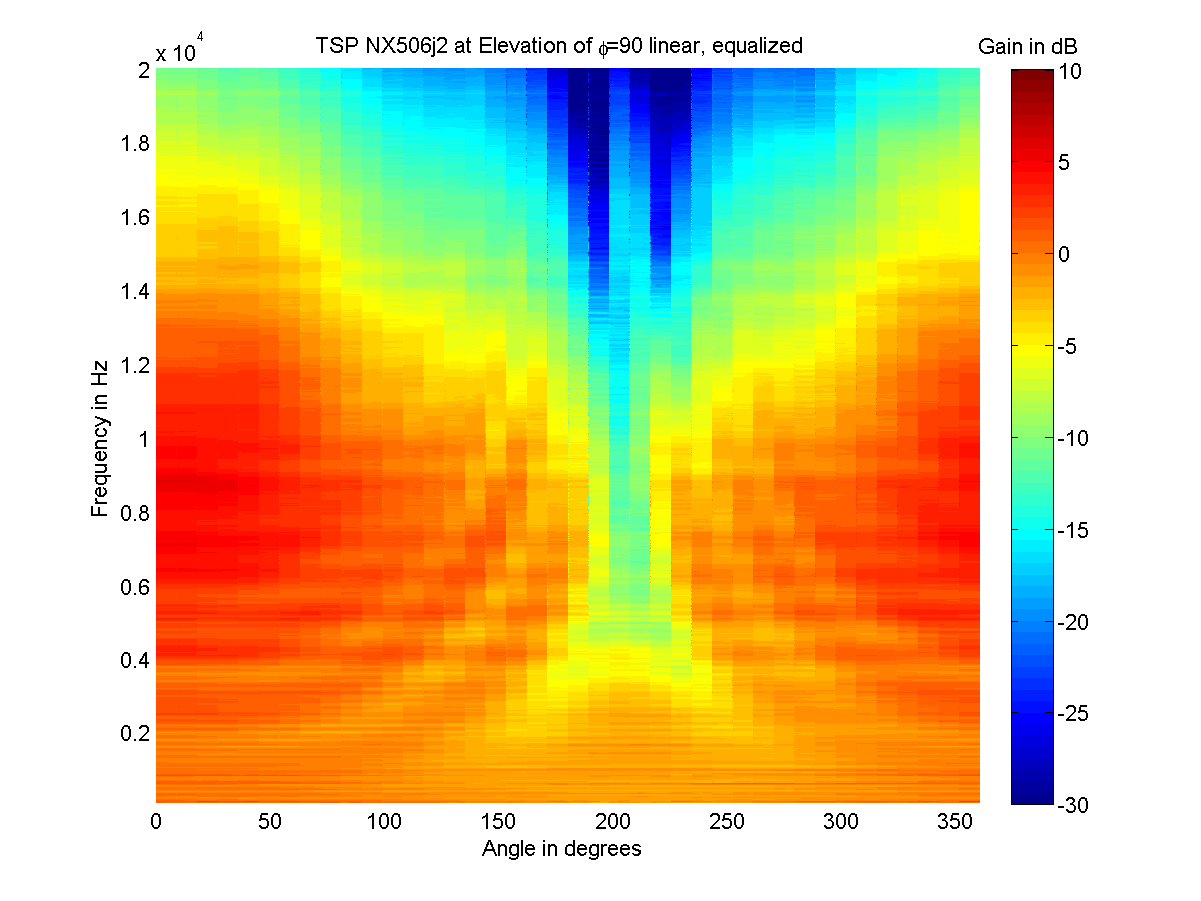
\includegraphics[height=0.28\textheight]{afbeeldingen/plots/results/NX506j2_TSP_090_lin_eq.png}
        \end{subfigure}~
        \begin{subfigure}[t]{0.5\textwidth}
			    \caption{$\phi=42^\circ$}
			    \label{fig:res_NX506_pluis_42}
                \centering
    			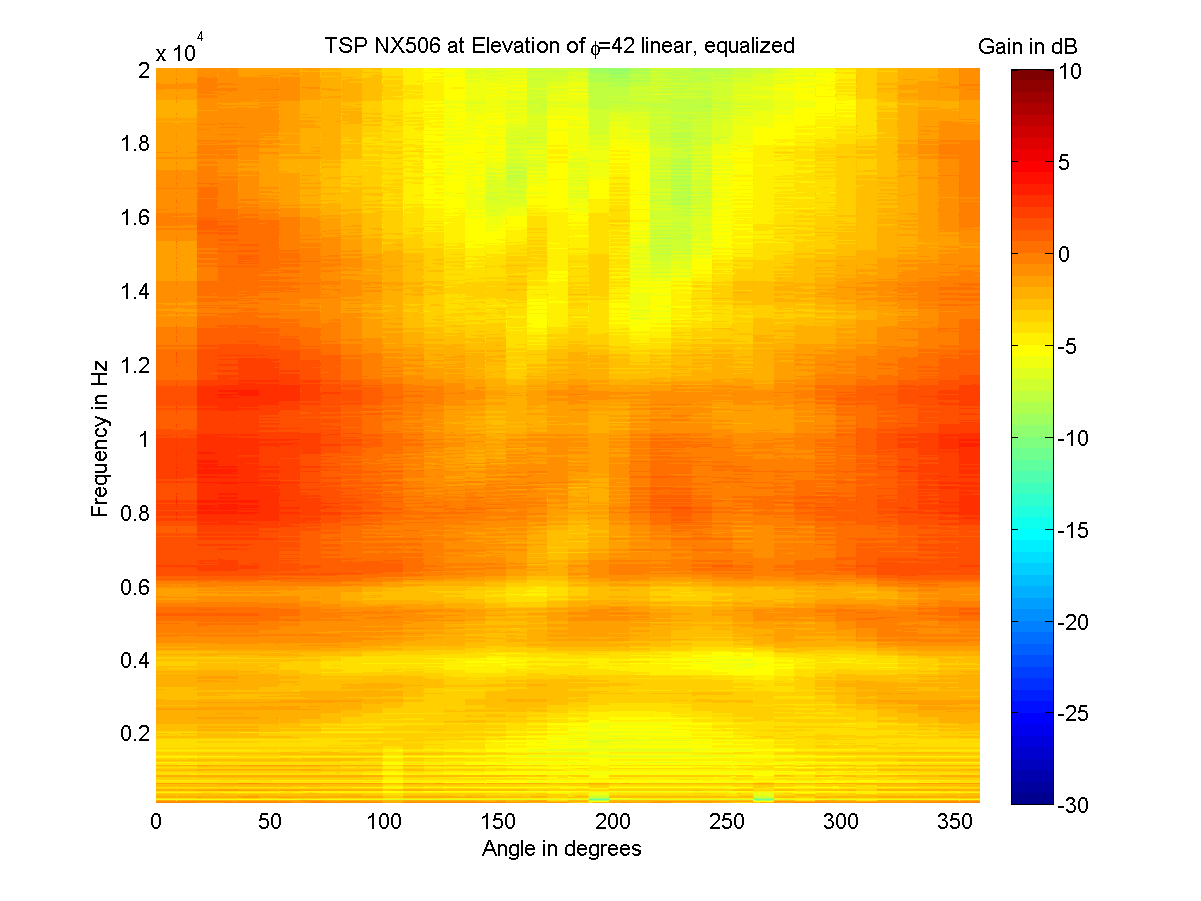
\includegraphics[height=0.28\textheight]{afbeeldingen/plots/results/NX506_TSP_042_lin_eq.png}
        \end{subfigure}
        
        \begin{subfigure}[t]{0.5\textwidth}
			    \caption{$\phi=138^\circ$}
			    \label{fig:res_NX506_pluis_138}
                \centering
    			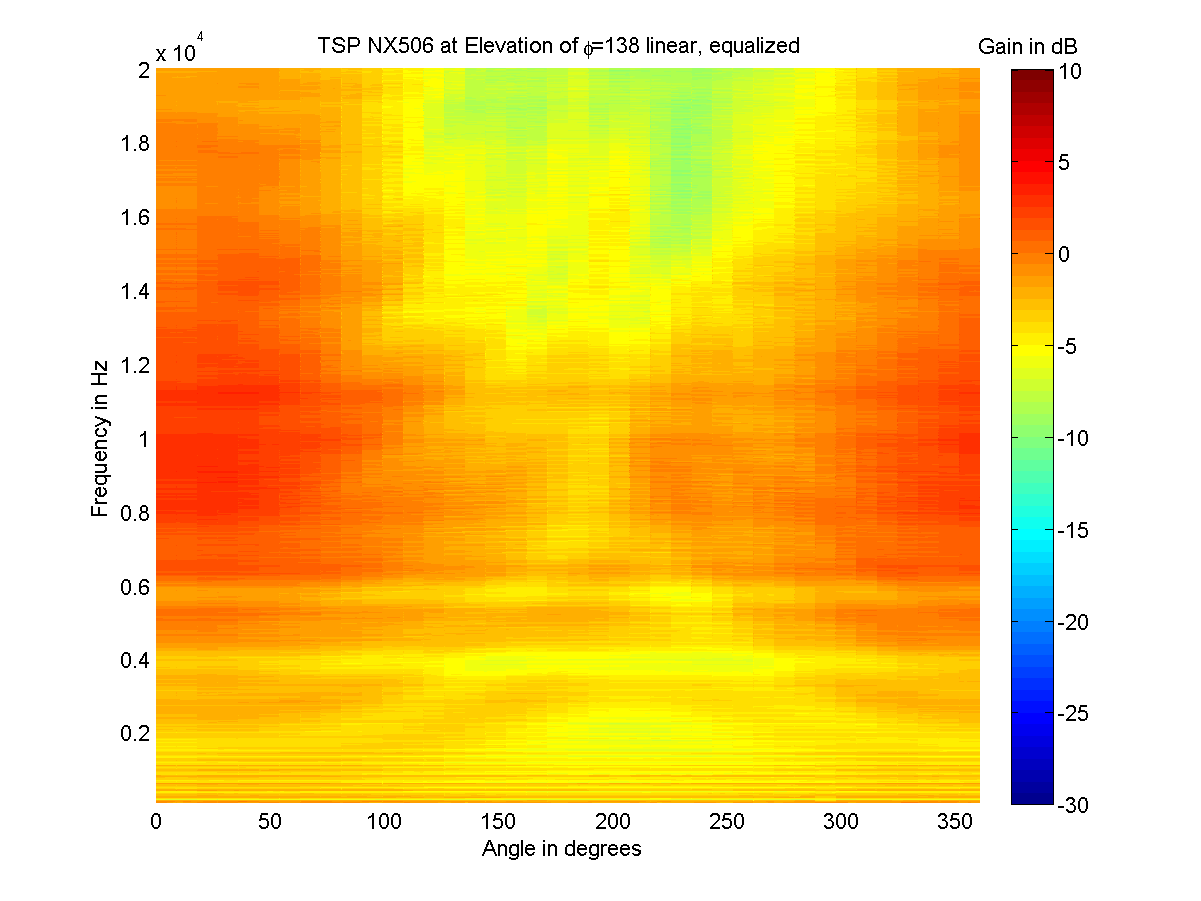
\includegraphics[height=0.28\textheight]{afbeeldingen/plots/results/NX506_TSP_138_lin_eq.png}
        \end{subfigure}~
        \begin{subfigure}[t]{0.5\textwidth}
			    \caption{North pole: $\phi=0^\circ$}
			    \label{fig:res_NX506_pluis_0}
                \centering
    			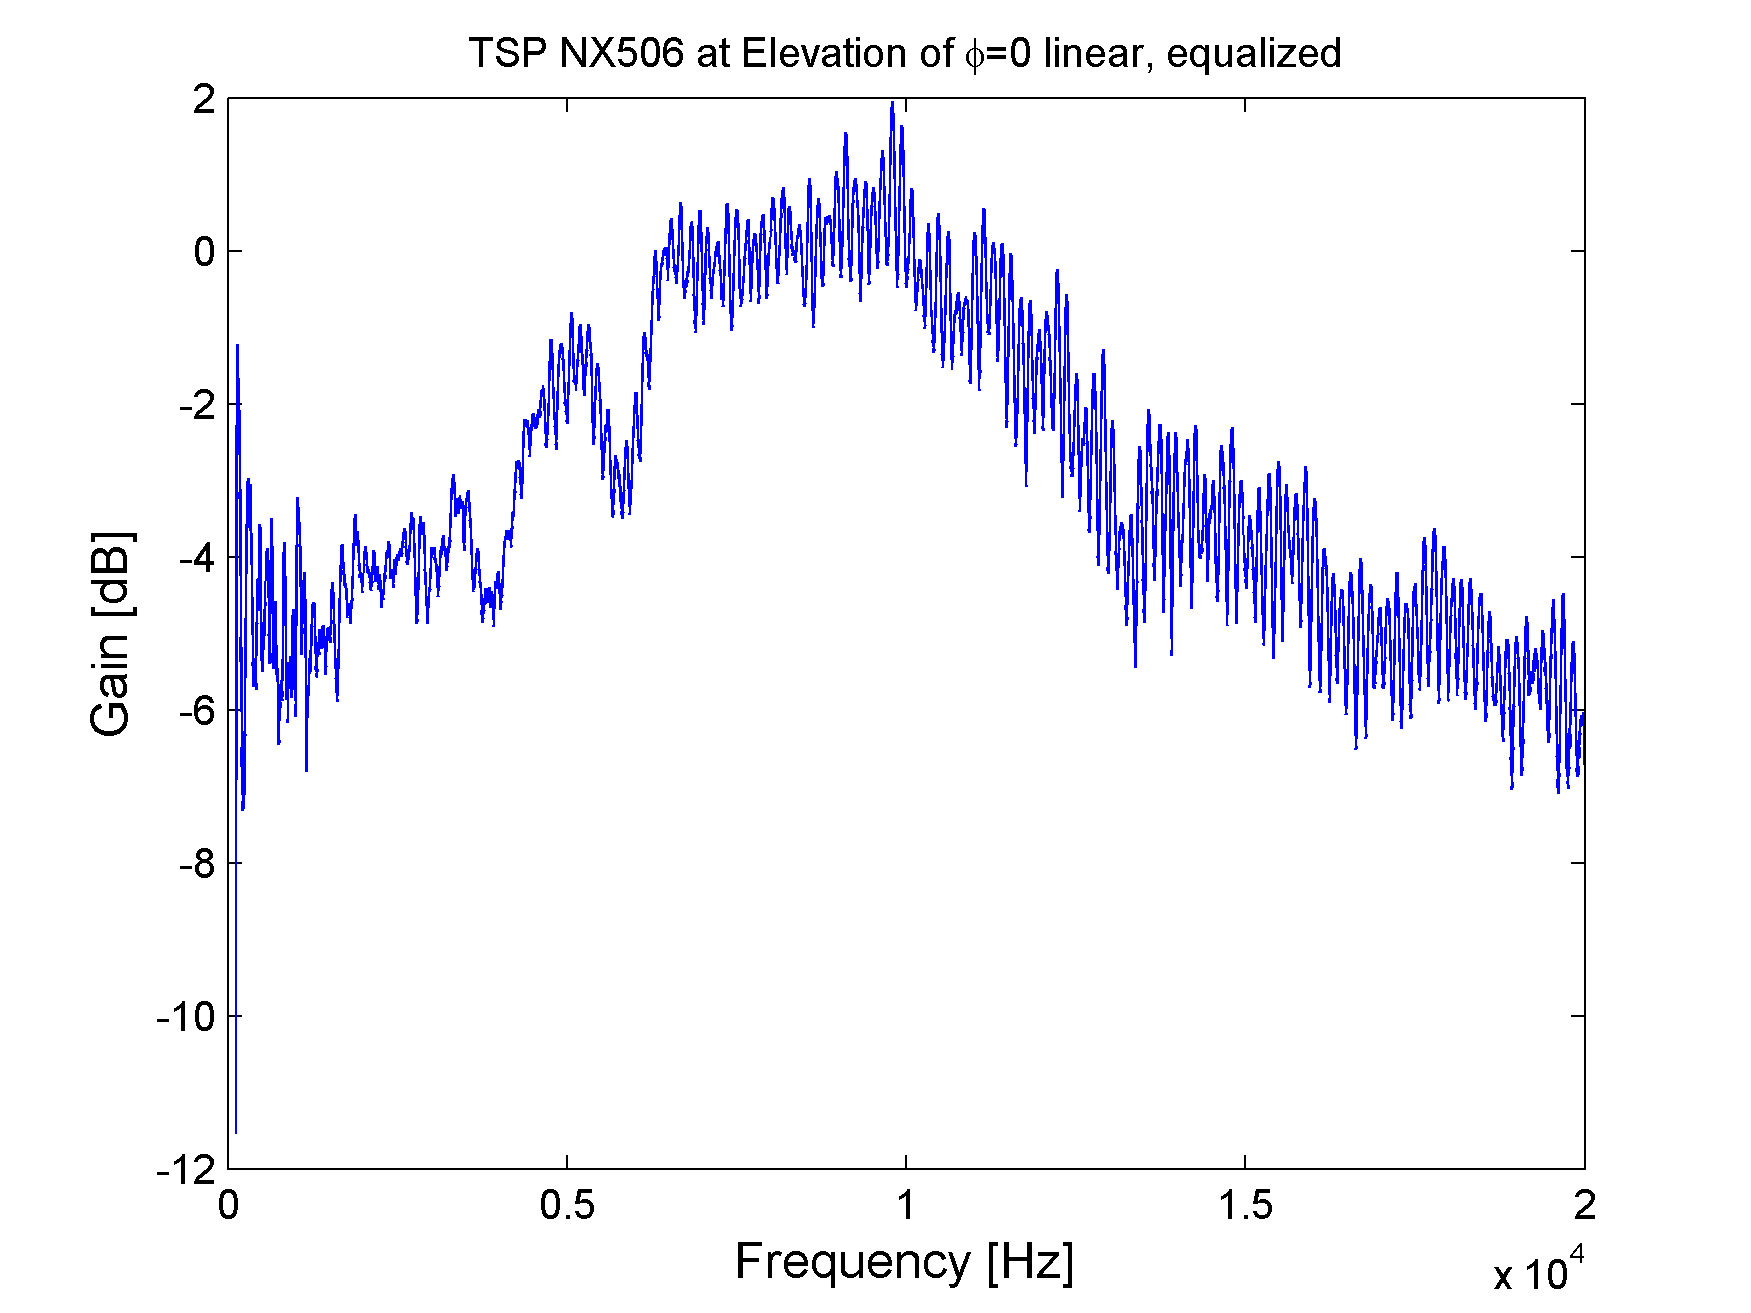
\includegraphics[height=0.28\textheight]{afbeeldingen/plots/results/NX506_north.png}
        \end{subfigure}
        
        \begin{subfigure}[t]{0.5\textwidth}
			    \caption{Full sphere $f=10000$ Hz, from the left}
			    \label{fig:res_NX506_pluis_sphere_left}
                \centering
    			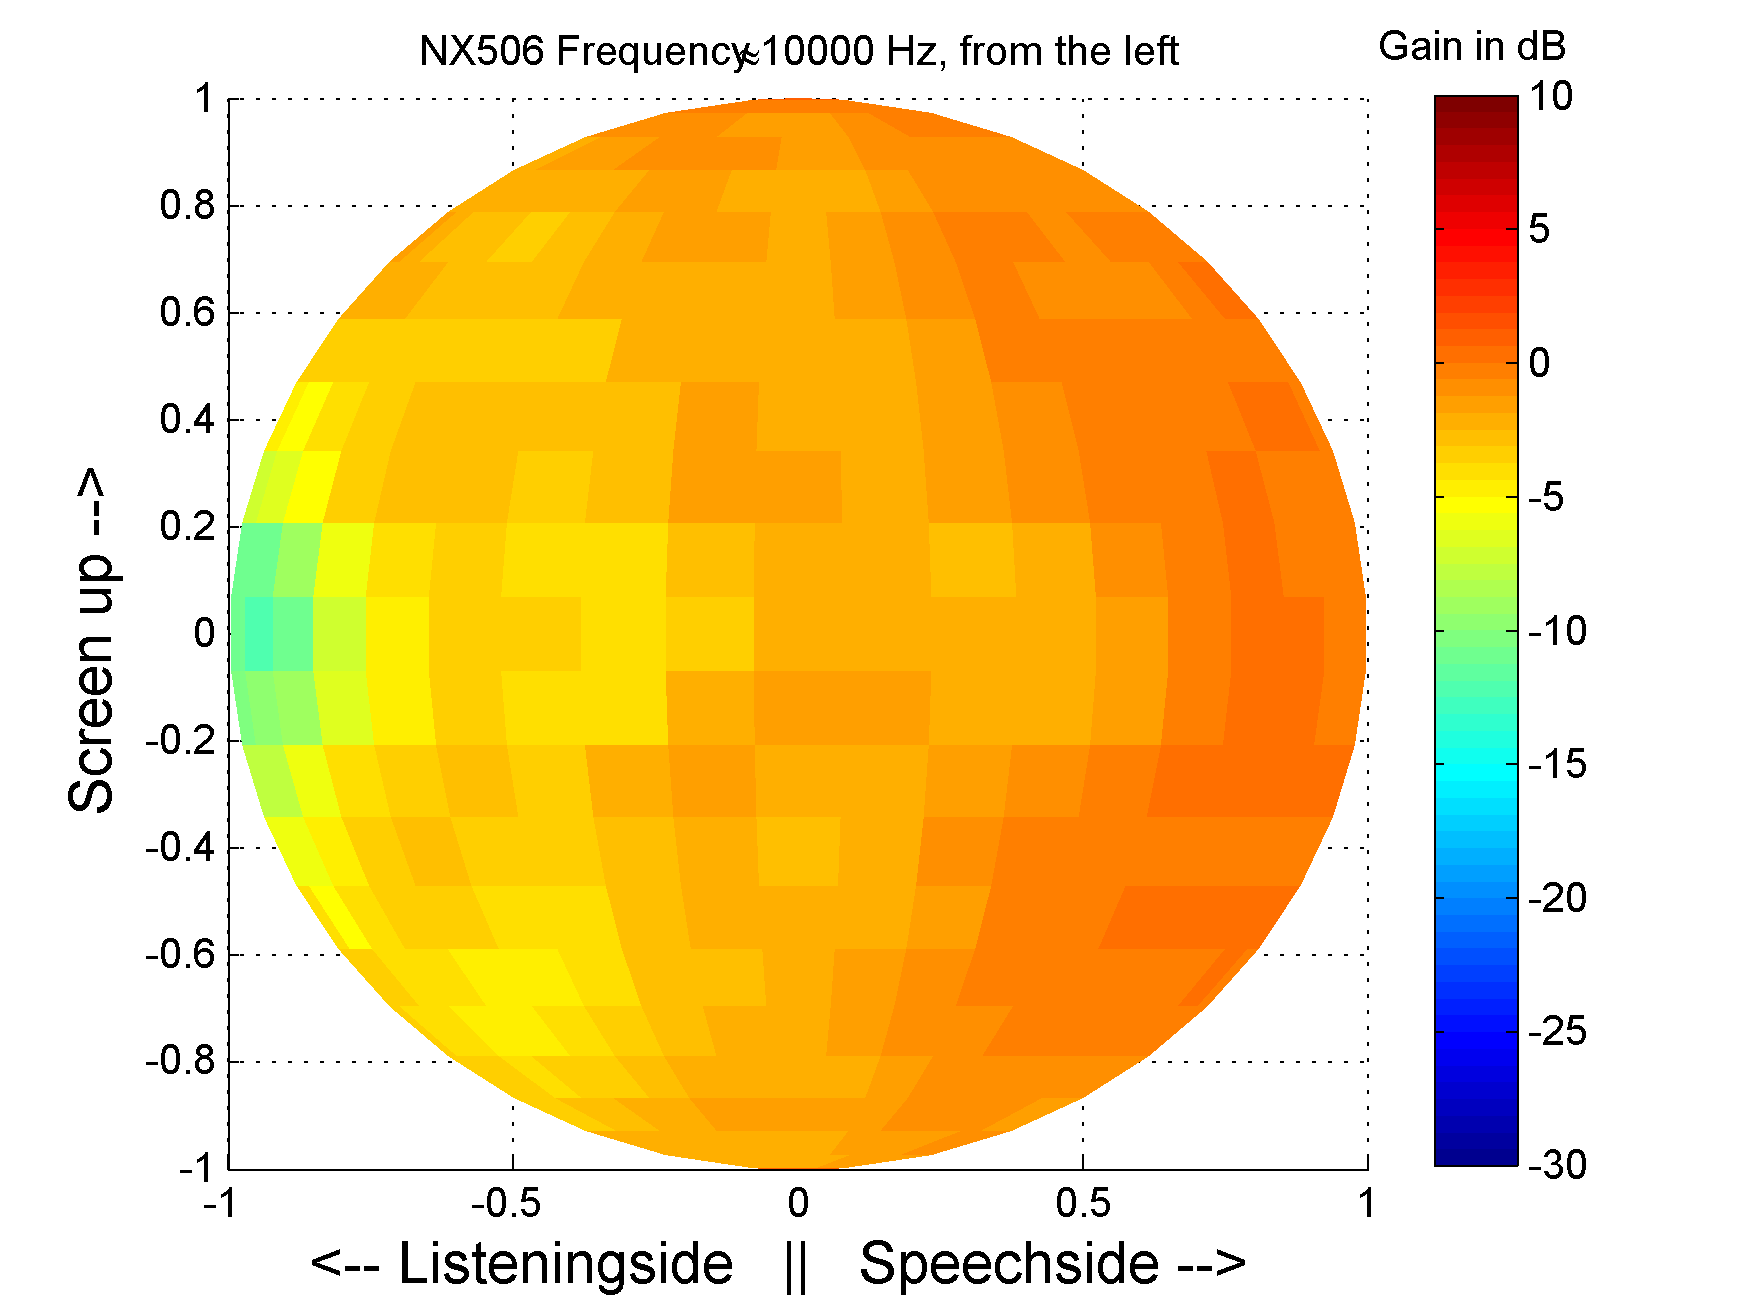
\includegraphics[height=0.28\textheight]{afbeeldingen/plots/results/NX506_10000_left.png}
        \end{subfigure}~
        \begin{subfigure}[t]{0.5\textwidth}
			    \caption{Full sphere $f=10000$ Hz, from the right}
			    \label{fig:res_NX506_pluis_sphere_right}
                \centering
    			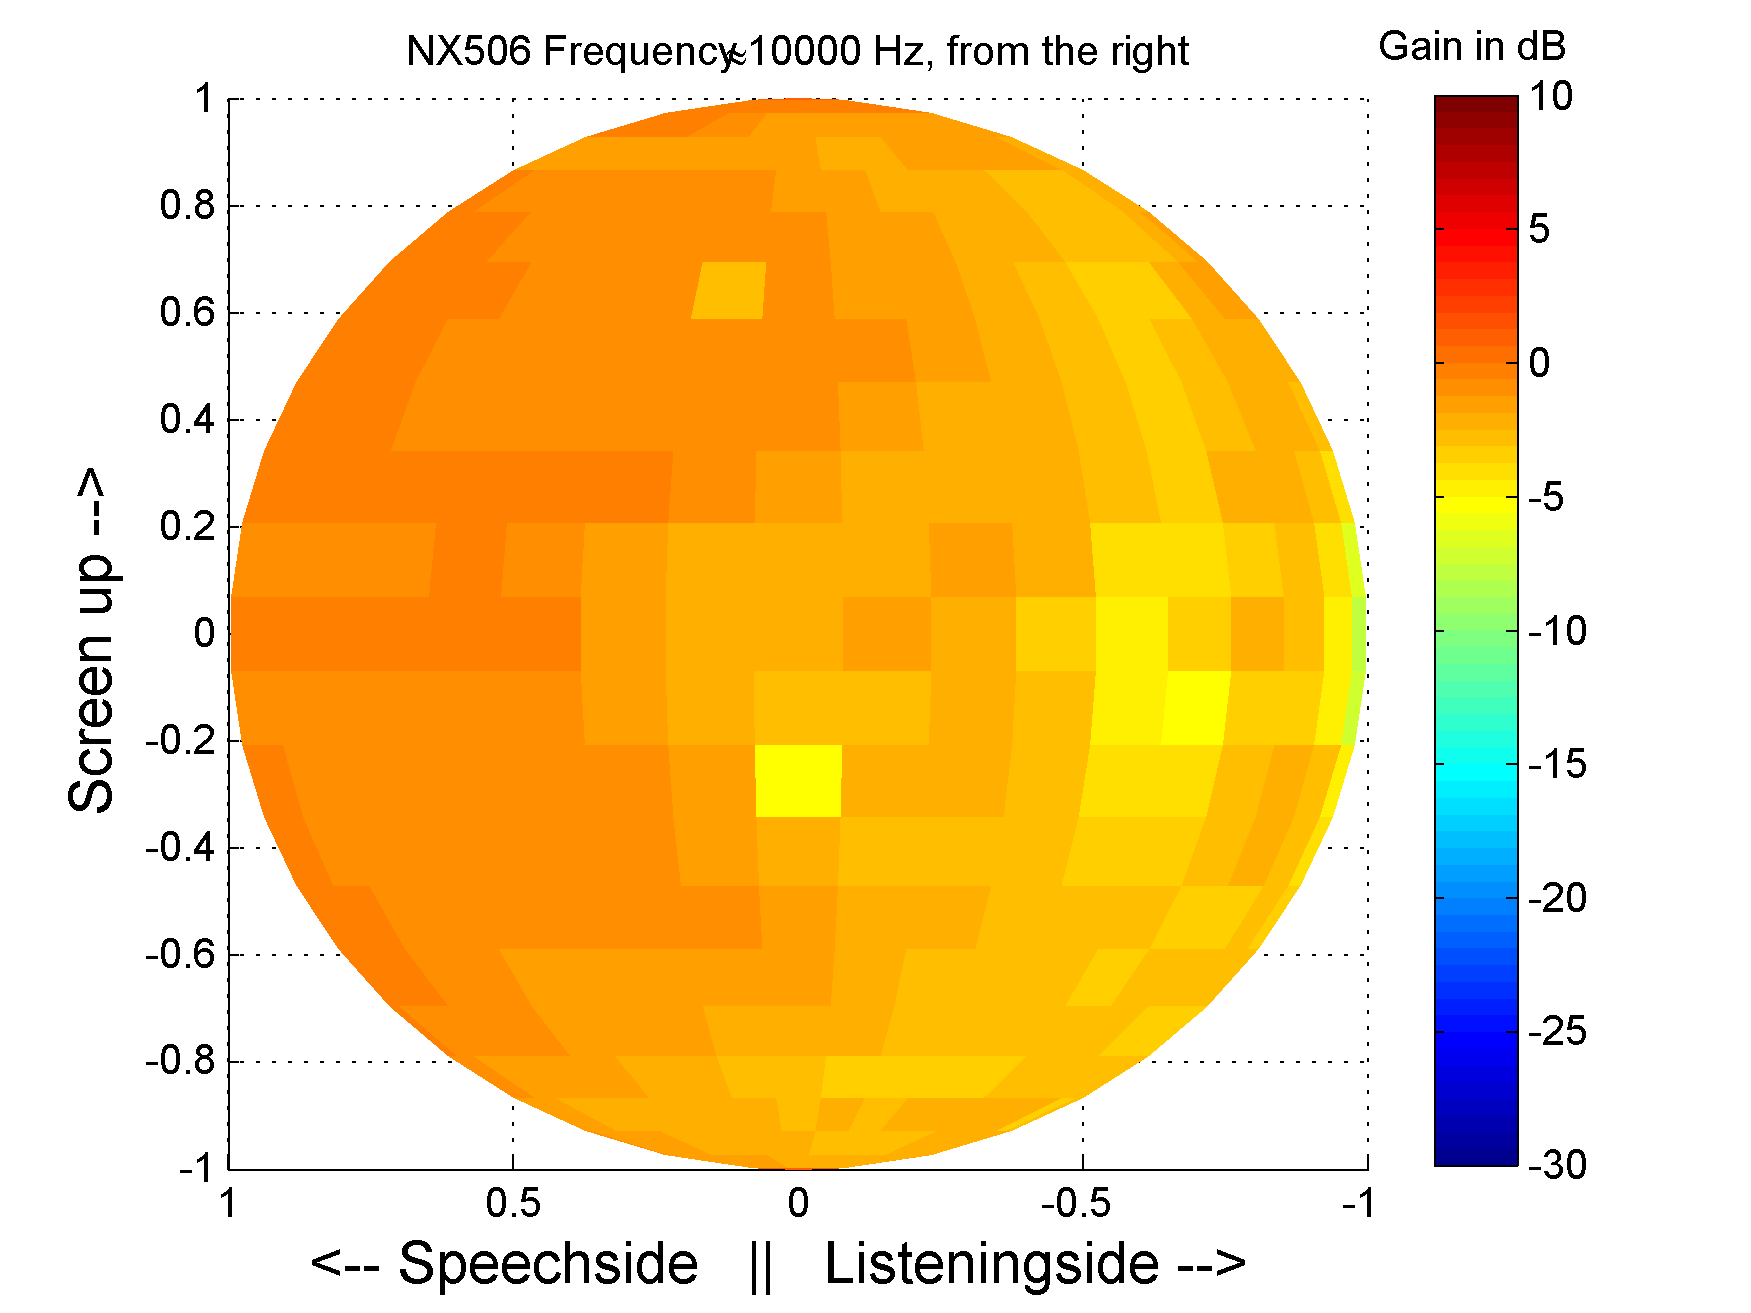
\includegraphics[height=0.28\textheight]{afbeeldingen/plots/results/NX506_10000_right.png}
        \end{subfigure}
\end{figure}

%%%%%%%%%%%%%%%%%%%%%%%%%%%%%%%%%%%%%%%%%%%%%%%%%%%%%%%%%%%%%%%%%%%%%%%%%%%%%%%%%%%%%%%%%%%%
% NX506 FU
\clearpage
\begin{figure}[t!]
        \centering
        
        \caption[Measurement results {\nexus} (6), face up]{{\nexus}, labelled with number 6, measurements in face up position, equalized}
        \label{fig:res_NX506_FU}

        \begin{subfigure}[t]{0.5\textwidth}
			    \caption{$\phi=90^\circ$}
			    \label{fig:res_NX506_FU_90}
                \centering
    			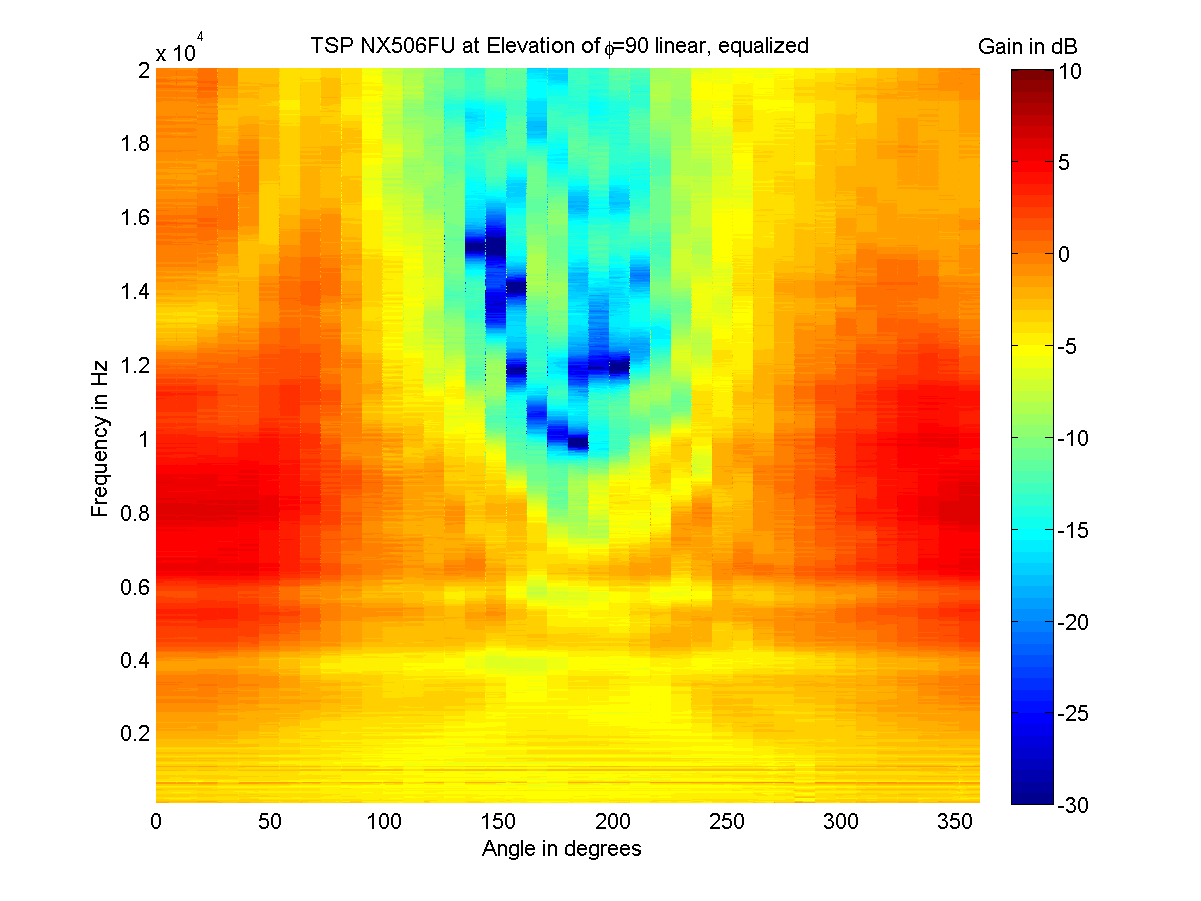
\includegraphics[height=0.28\textheight]{afbeeldingen/plots/results/NX506FU_TSP_090_lin_eq.png}
        \end{subfigure}~
        \begin{subfigure}[t]{0.5\textwidth}
			    \caption{$\phi=45^\circ$}
			    \label{fig:res_NX506_FU_45}
                \centering
    			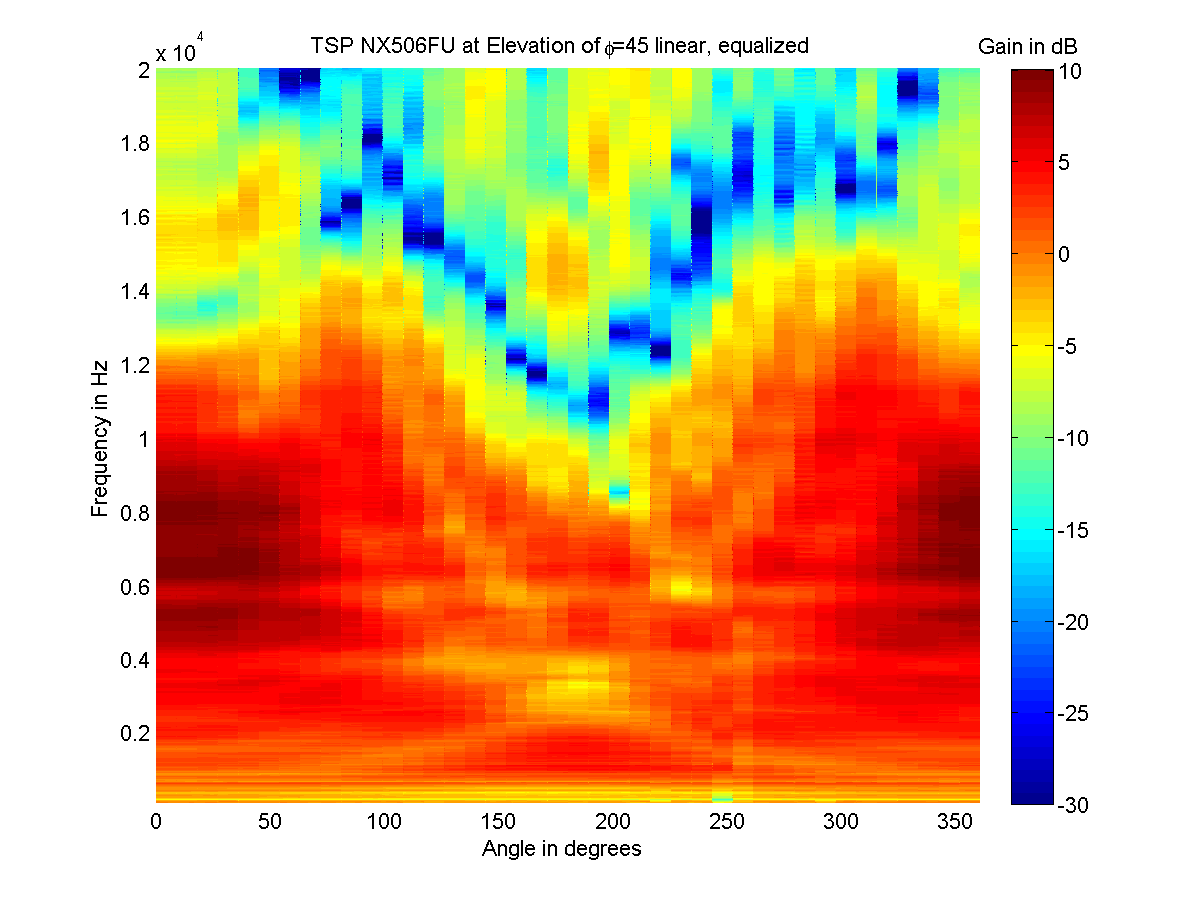
\includegraphics[height=0.28\textheight]{afbeeldingen/plots/results/NX506FU_TSP_045_lin_eq.png}
        \end{subfigure}
        
        \begin{subfigure}[t]{0.5\textwidth}
			    \caption{$\phi=135^\circ$}
			    \label{fig:res_NX506_FU_135}
                \centering
    			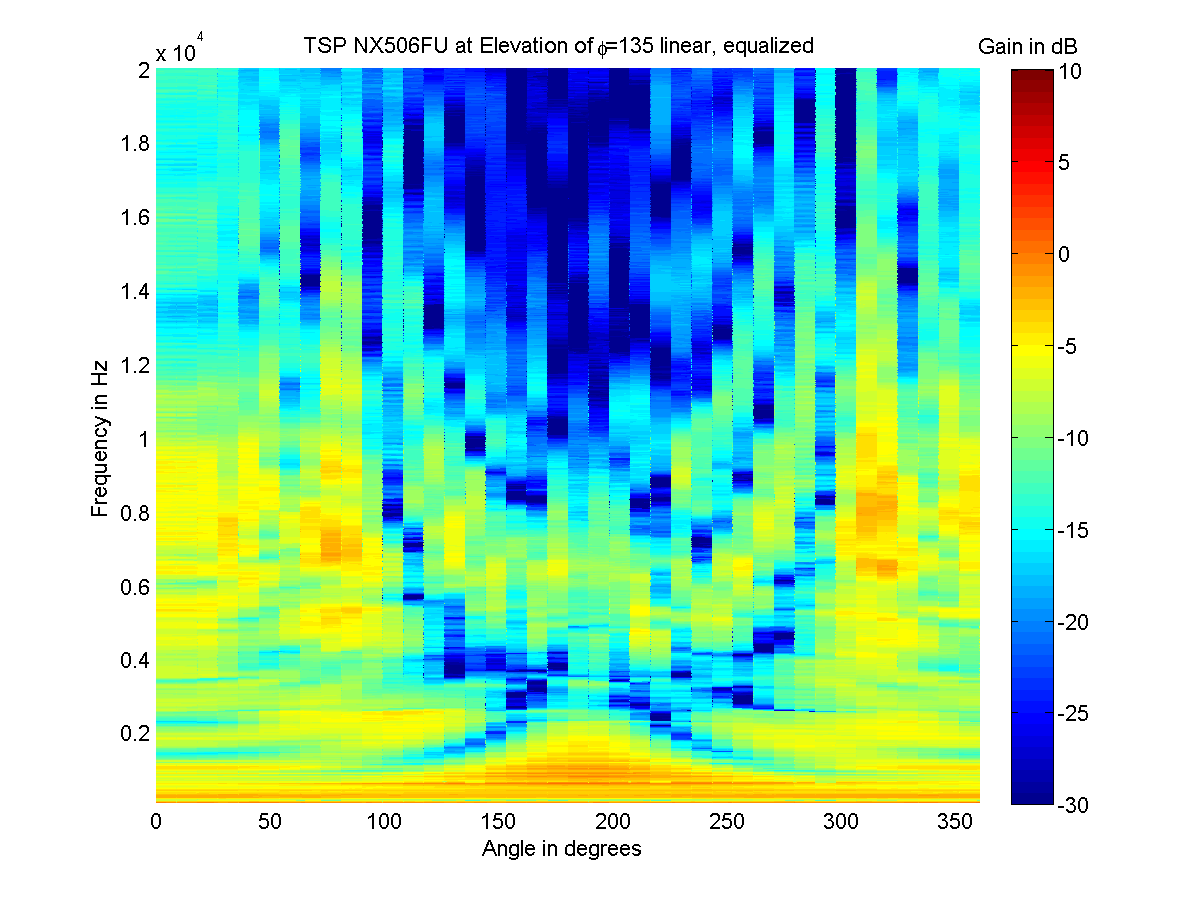
\includegraphics[height=0.28\textheight]{afbeeldingen/plots/results/NX506FU_TSP_135_lin_eq.png}
        \end{subfigure}~
        \begin{subfigure}[t]{0.5\textwidth}
			    \caption{North pole: $\phi=0^\circ$}
			    \label{fig:res_NX506_FU_0}
                \centering
    			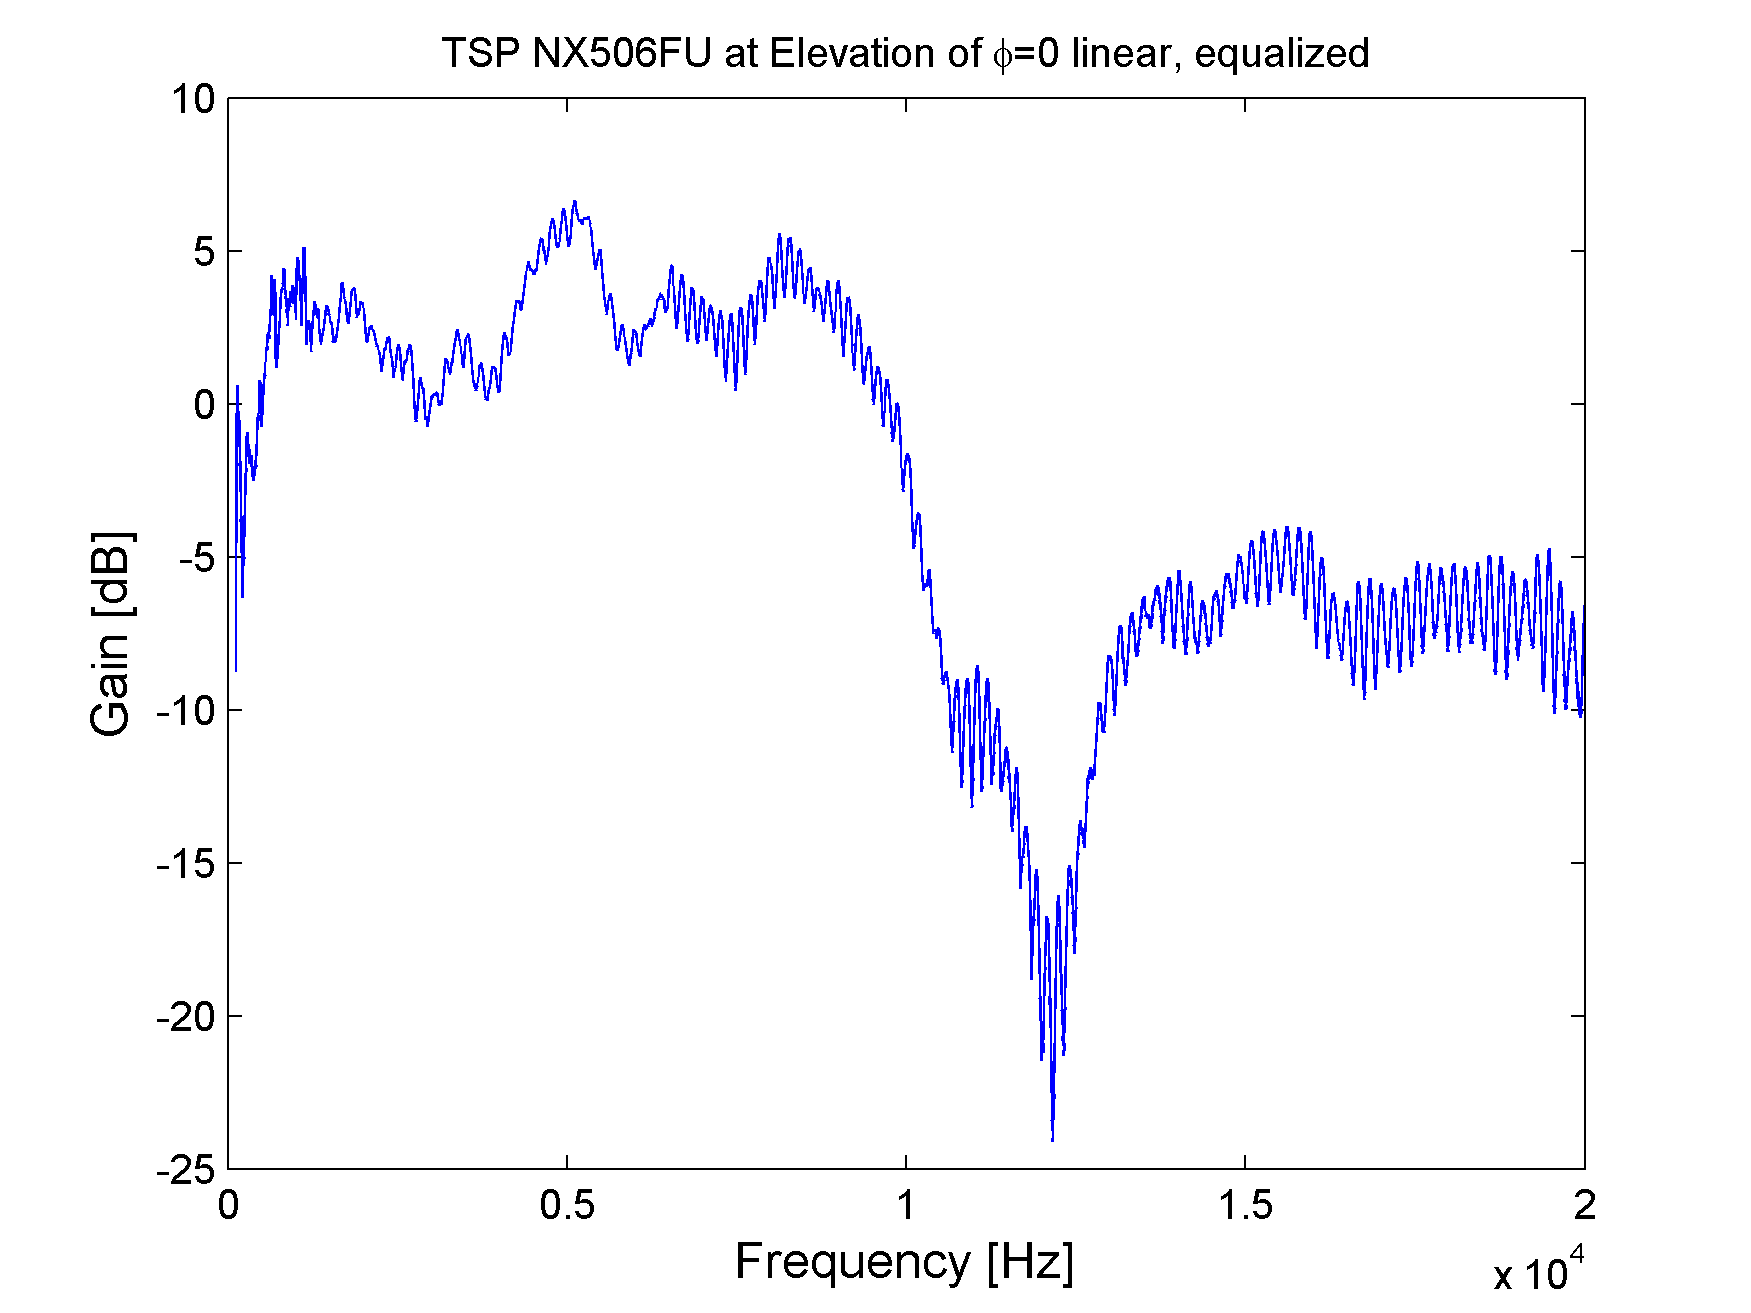
\includegraphics[height=0.28\textheight]{afbeeldingen/plots/results/NX506FU_north.png}
        \end{subfigure}
        
        \begin{subfigure}[t]{0.5\textwidth}
			    \caption{Full sphere $f=10000$ Hz, from the left}
			    \label{fig:res_NX506_FU_sphere_left}
                \centering
    			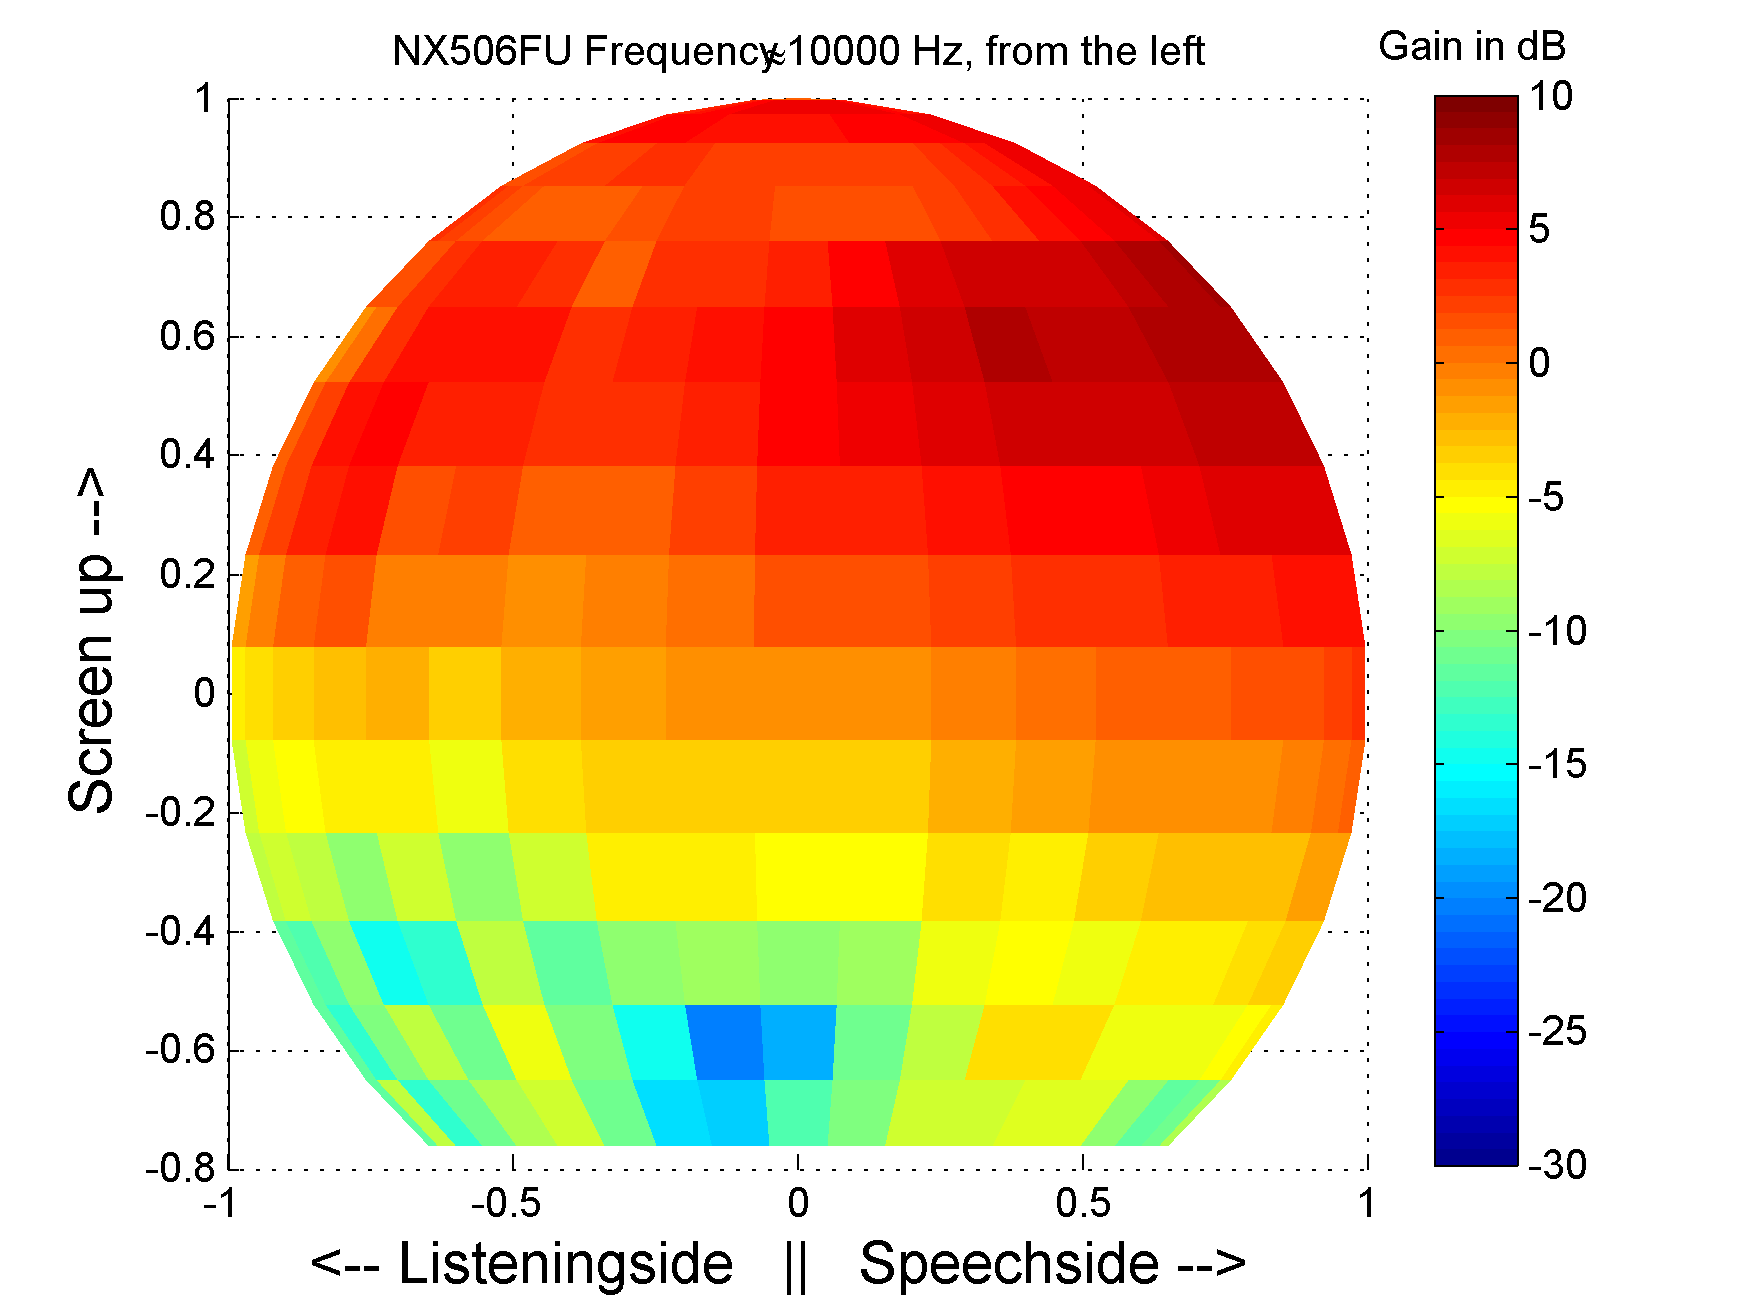
\includegraphics[height=0.28\textheight]{afbeeldingen/plots/results/NX506FU_10000_left.png}
        \end{subfigure}~
        \begin{subfigure}[t]{0.5\textwidth}
			    \caption{Full sphere $f=10000$ Hz, from the right}
			    \label{fig:res_NX506_FU_sphere_right}
                \centering
    			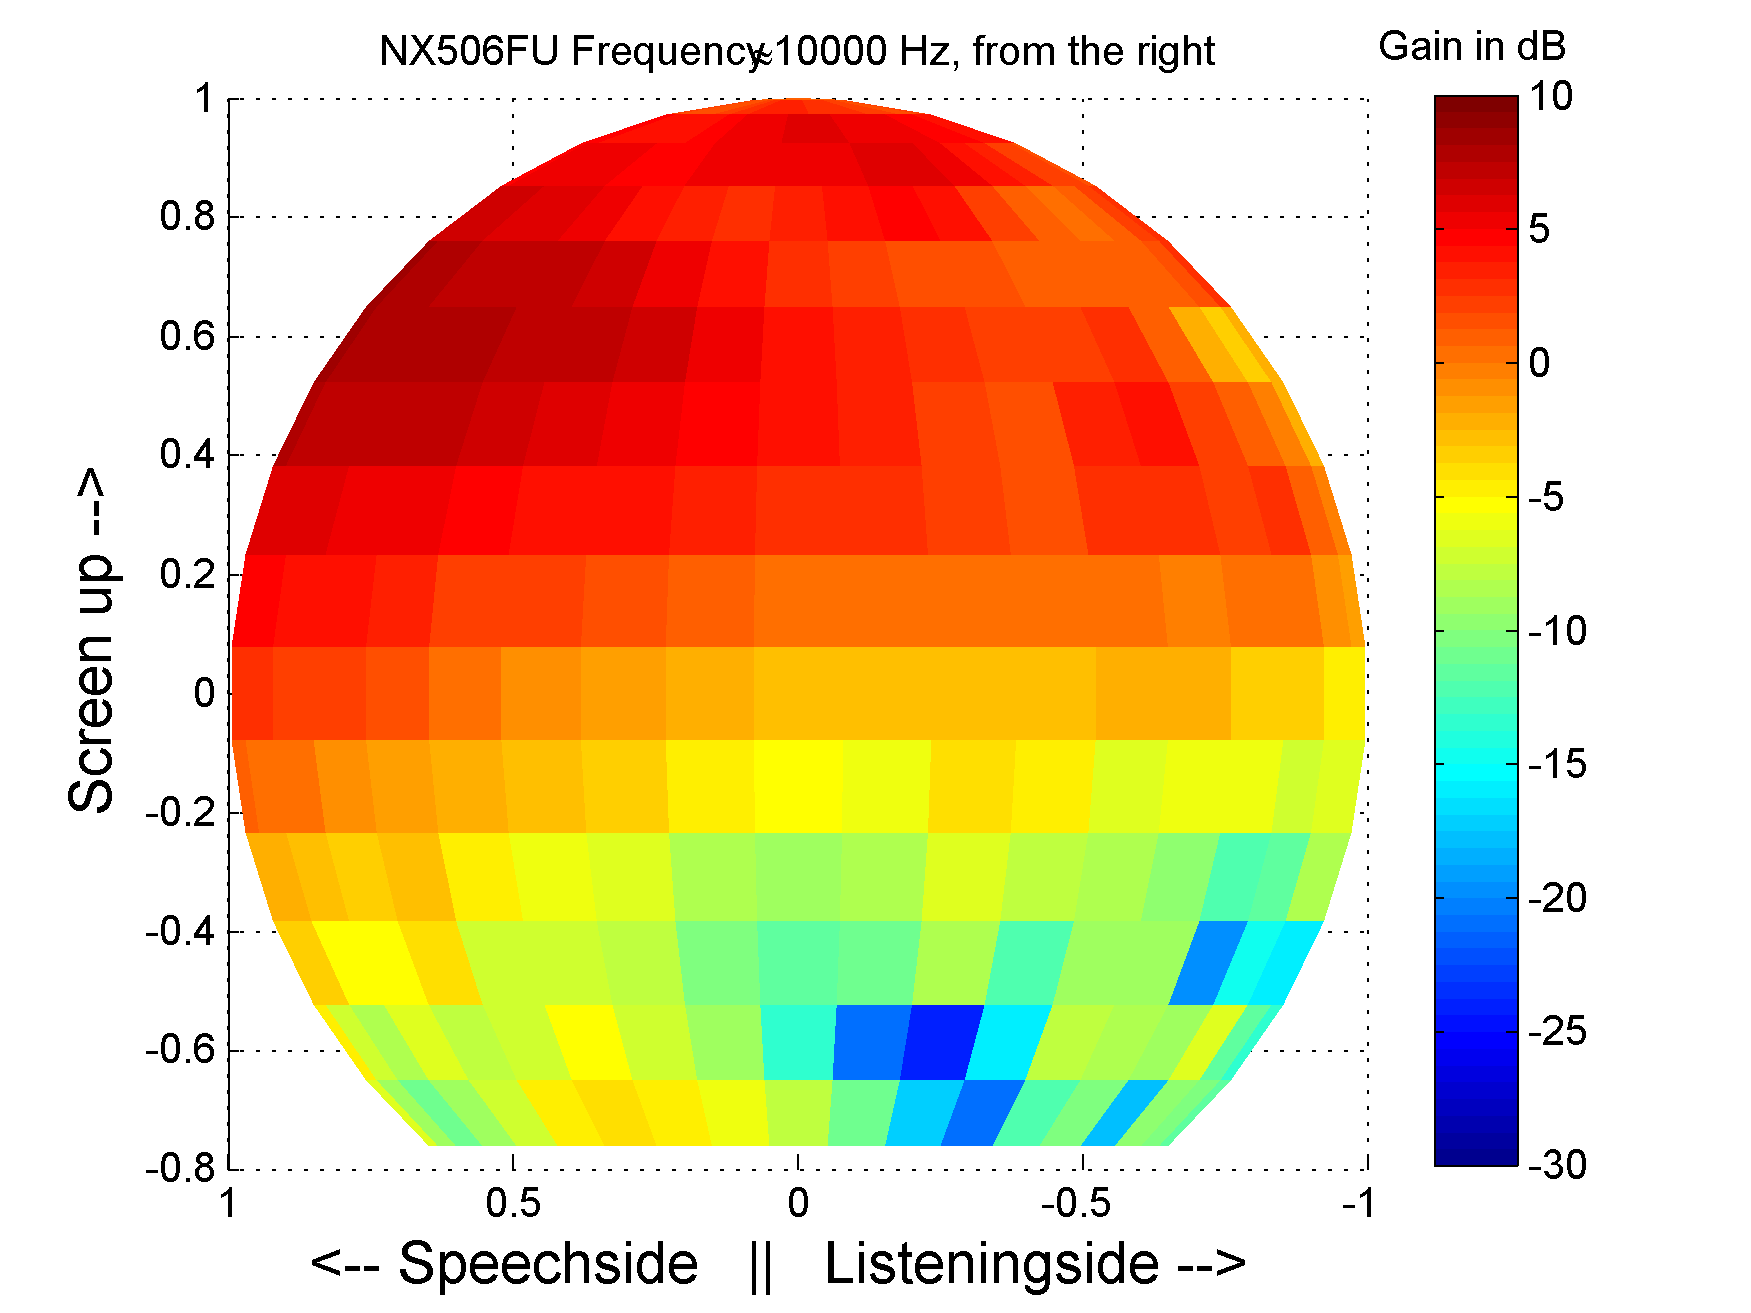
\includegraphics[height=0.28\textheight]{afbeeldingen/plots/results/NX506FU_10000_right.png}
        \end{subfigure}
\end{figure}

%%%%%%%%%%%%%%%%%%%%%%%%%%%%%%%%%%%%%%%%%%%%%%%%%%%%%%%%%%%%%%%%%%%%%%%%%%%%%%%%%%%%%%%%%%%%
% NX506 FD
\clearpage
\begin{figure}[t!]
        \centering
        
        \caption[Measurement results {\nexus} (6), face down]{{\nexus}, labelled with number 6, measurements in face down position, equalized}
        \label{fig:res_NX506_FD}

        \begin{subfigure}[t]{0.5\textwidth}
			    \caption{$\phi=90^\circ$}
			    \label{fig:res_NX506_FD_90}
                \centering
    			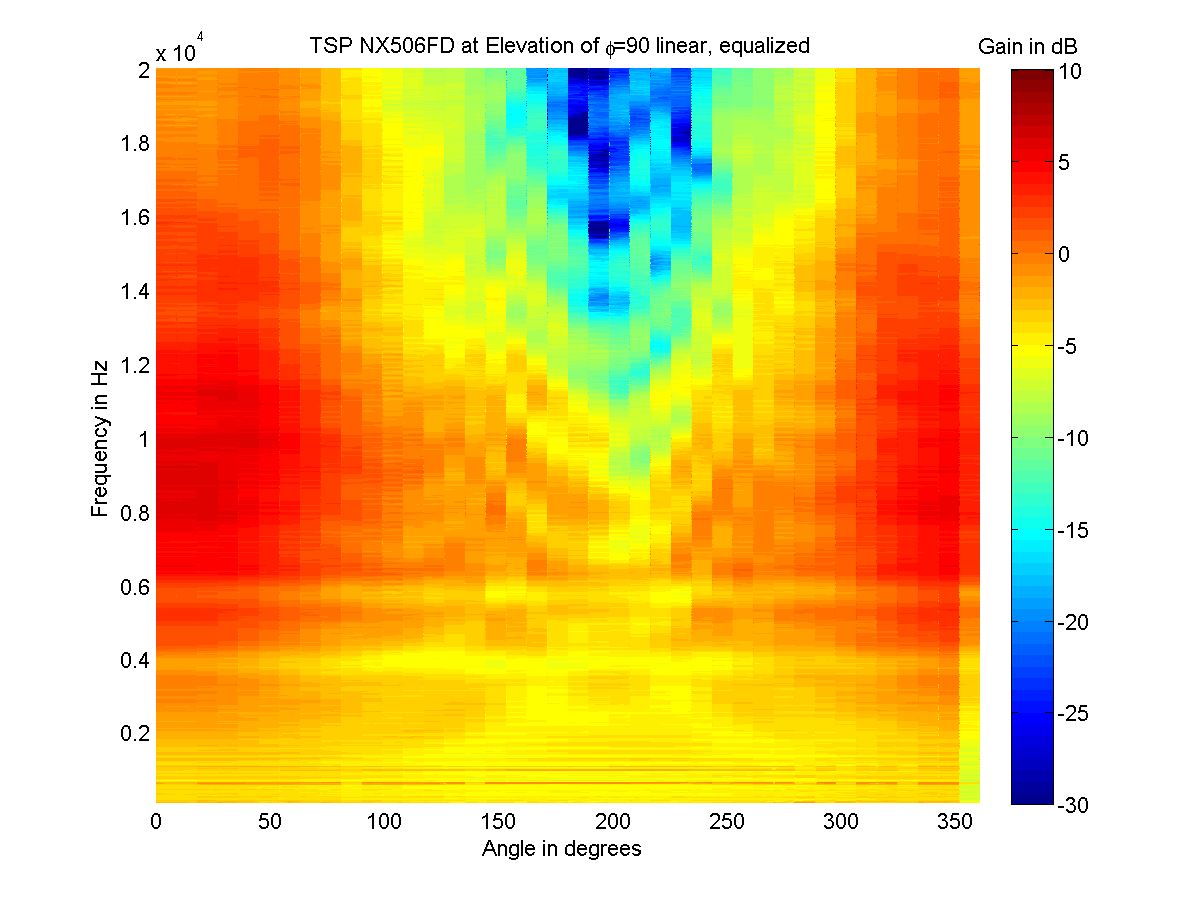
\includegraphics[height=0.28\textheight]{afbeeldingen/plots/results/NX506FD_TSP_090_lin_eq.png}
        \end{subfigure}~
        \begin{subfigure}[t]{0.5\textwidth}
			    \caption{$\phi=45^\circ$}
			    \label{fig:res_NX506_FD_45}
                \centering
    			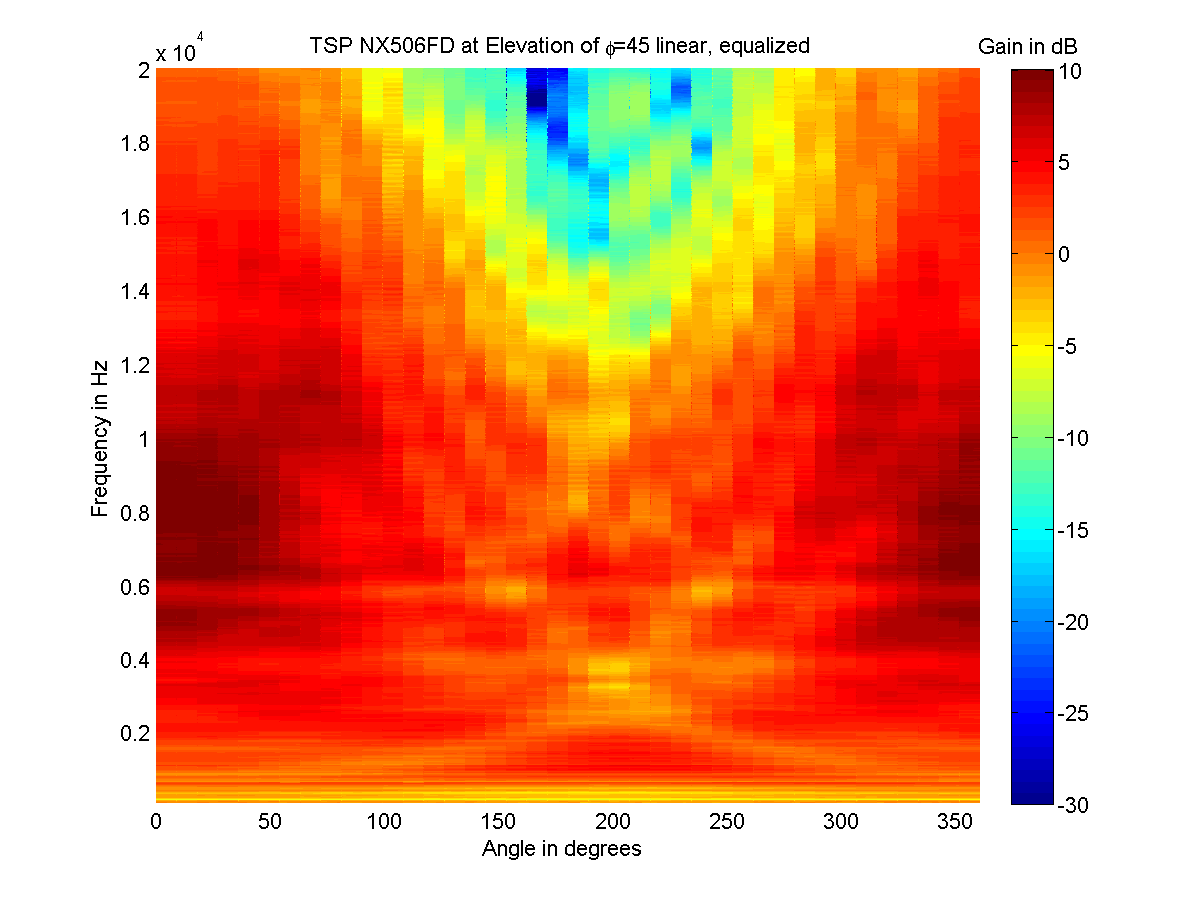
\includegraphics[height=0.28\textheight]{afbeeldingen/plots/results/NX506FD_TSP_045_lin_eq.png}
        \end{subfigure}
        
        \begin{subfigure}[t]{0.5\textwidth}
			    \caption{$\phi=135^\circ$}
			    \label{fig:res_NX506_FD_135}
                \centering
    			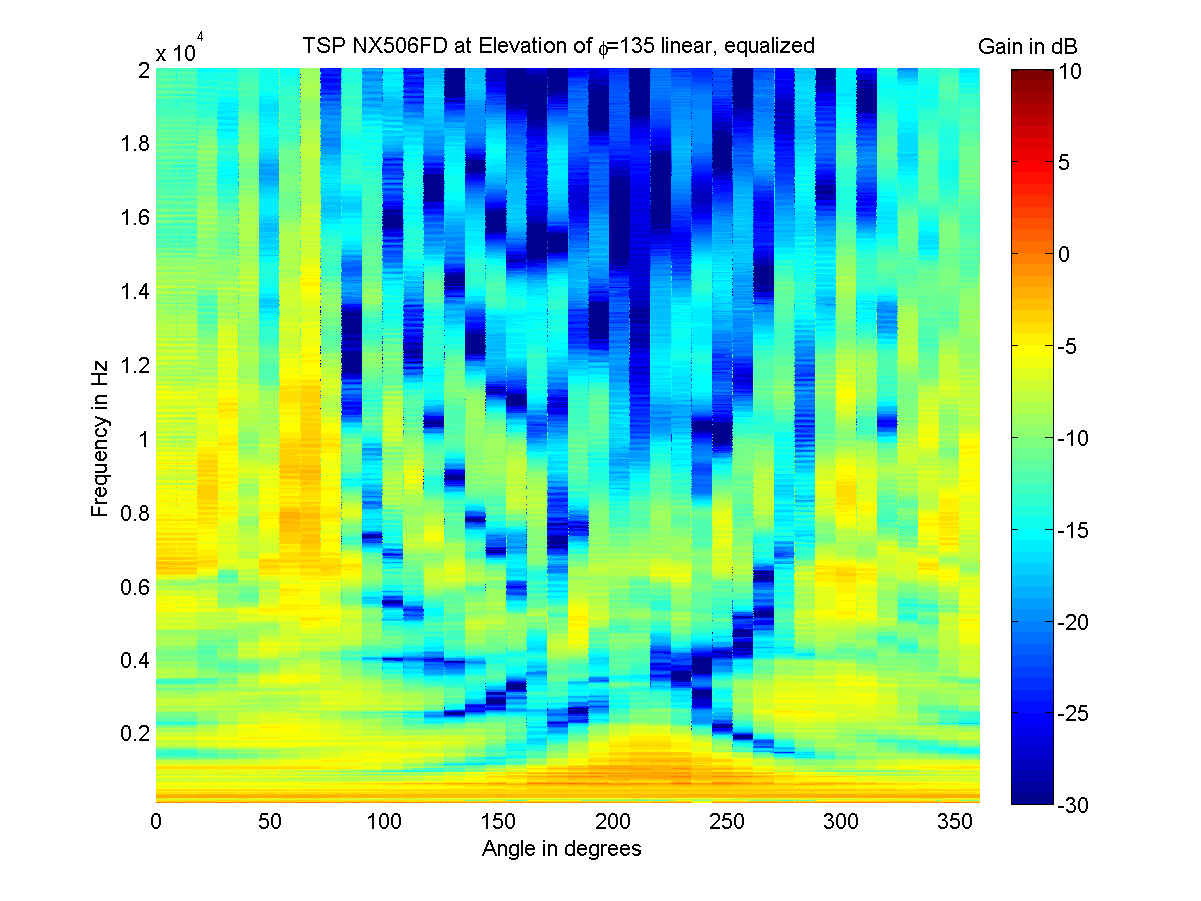
\includegraphics[height=0.28\textheight]{afbeeldingen/plots/results/NX506FD_TSP_135_lin_eq.png}
        \end{subfigure}~
        \begin{subfigure}[t]{0.5\textwidth}
			    \caption{North pole: $\phi=0^\circ$}
			    \label{fig:res_NX506_FD_0}
                \centering
    			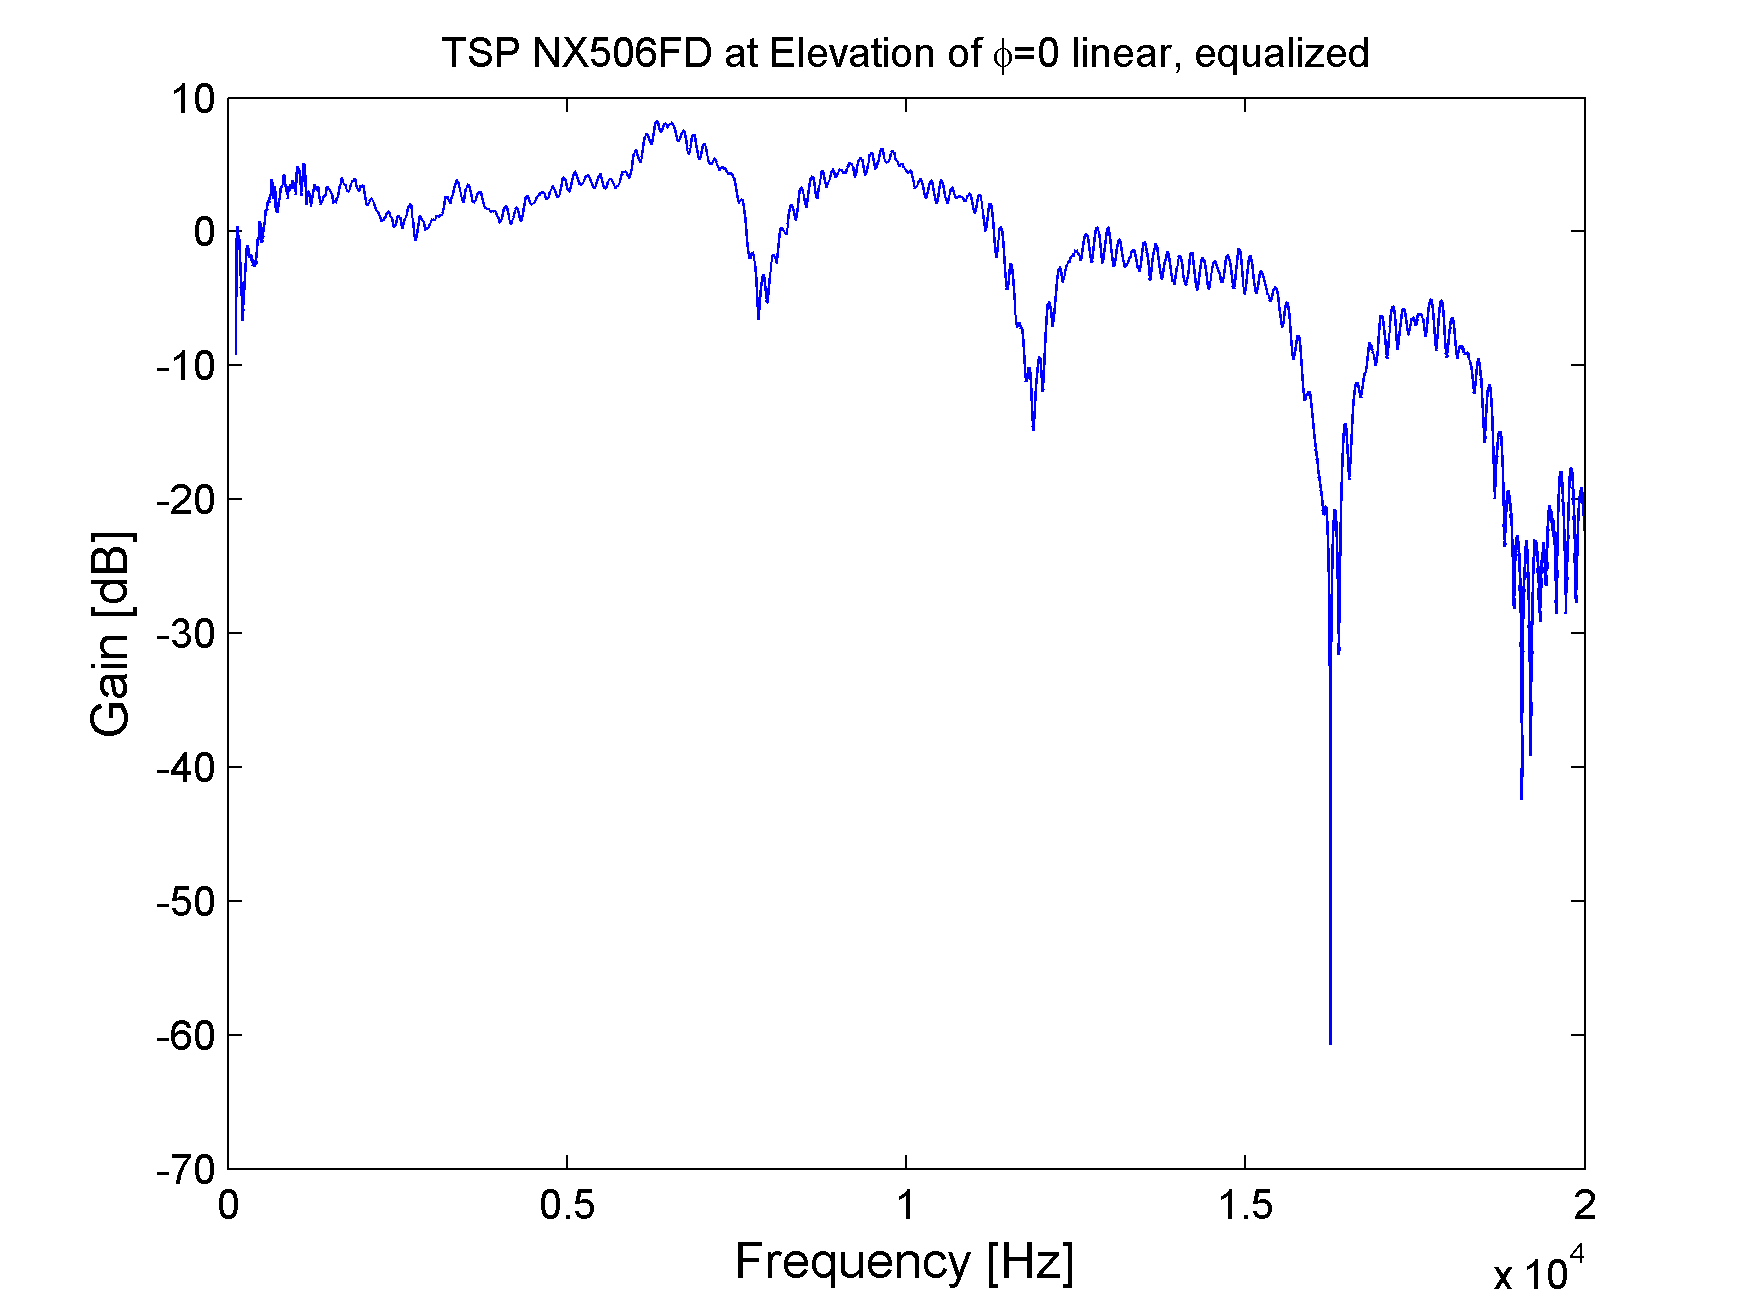
\includegraphics[height=0.28\textheight]{afbeeldingen/plots/results/NX506FD_north.png}
        \end{subfigure}
        
        \begin{subfigure}[t]{0.5\textwidth}
			    \caption{Full sphere $f=10000$ Hz, from the left}
			    \label{fig:res_NX506_FD_sphere_left}
                \centering
    			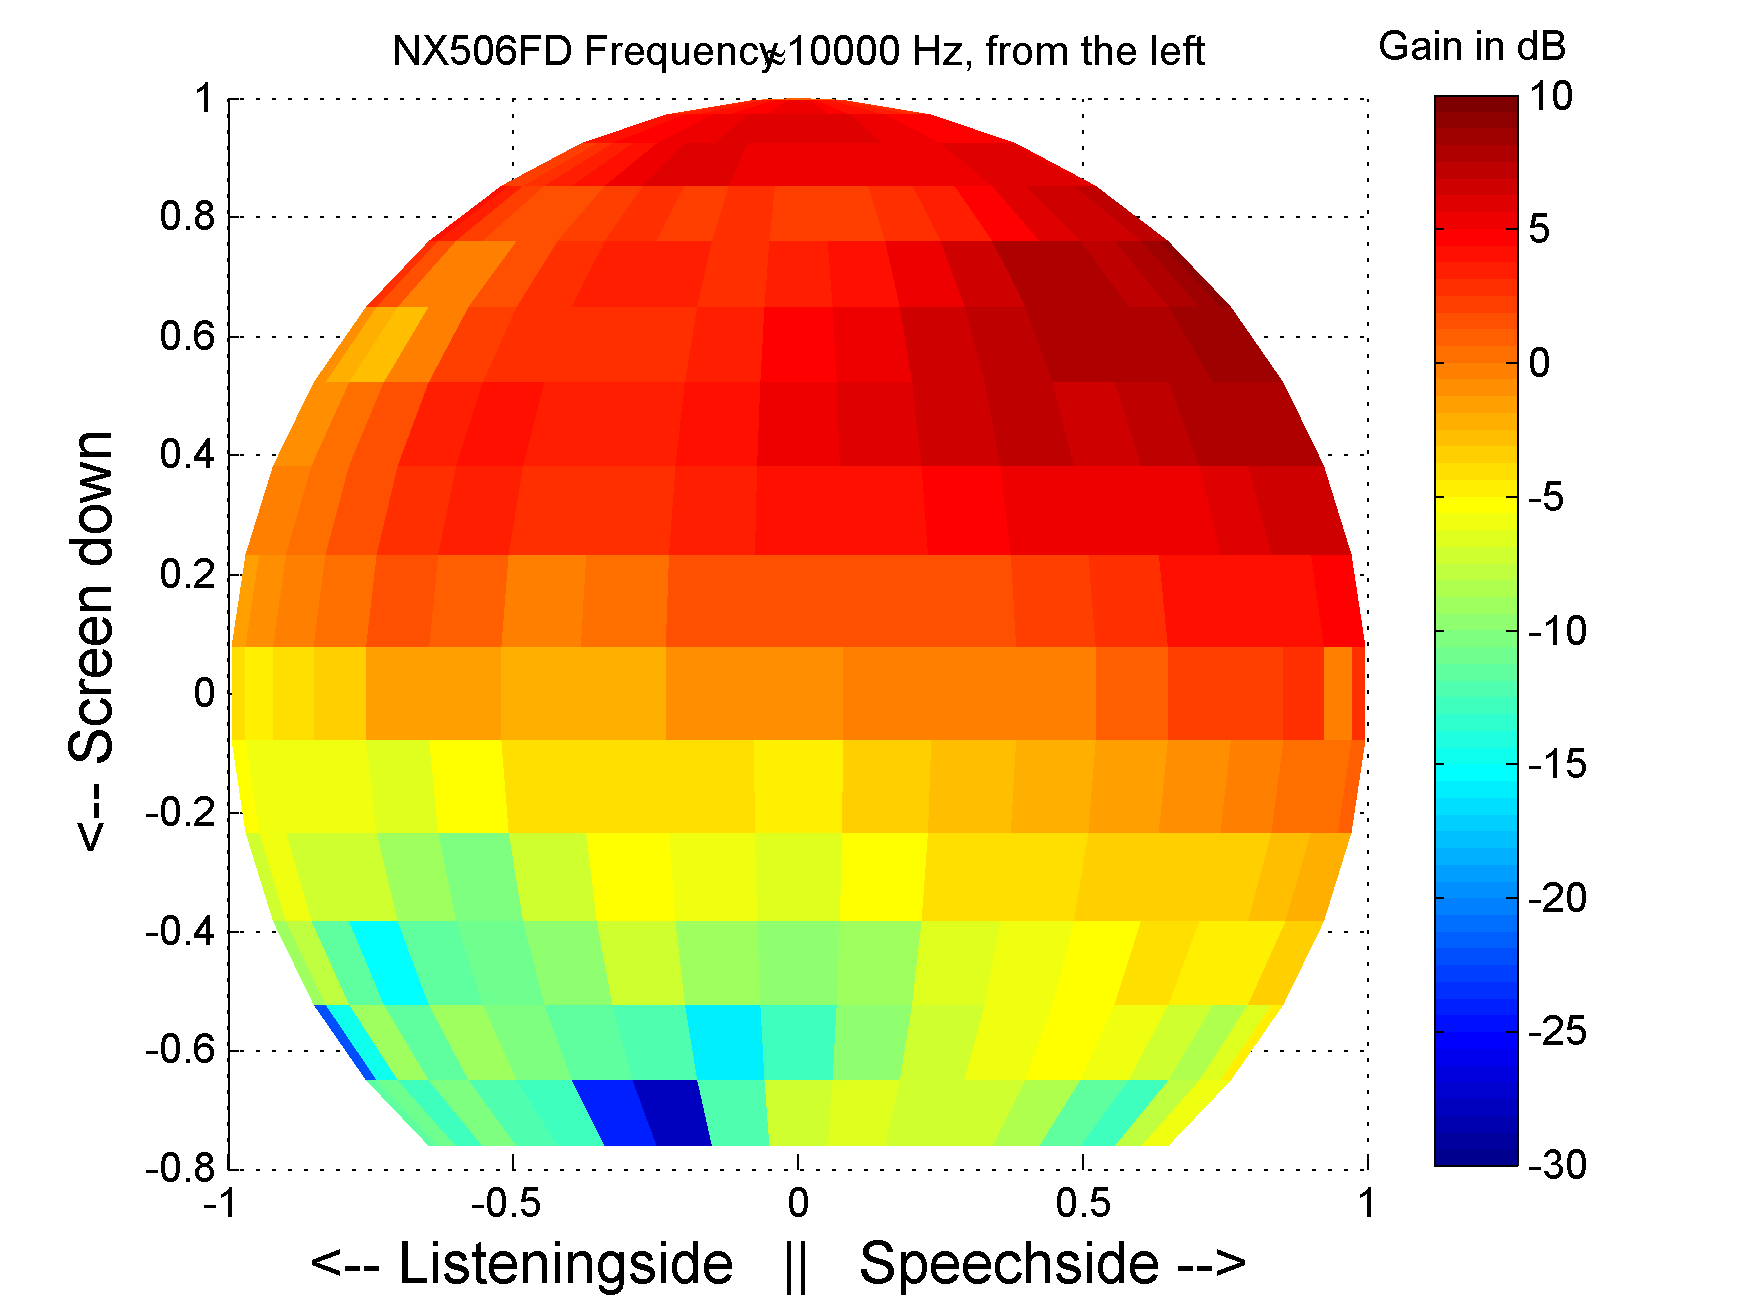
\includegraphics[height=0.28\textheight]{afbeeldingen/plots/results/NX506FD_10000_left.png}
        \end{subfigure}~
        \begin{subfigure}[t]{0.5\textwidth}
			    \caption{Full sphere $f=10000$ Hz, from the right}
			    \label{fig:res_NX506_FD_sphere_right}
                \centering
    			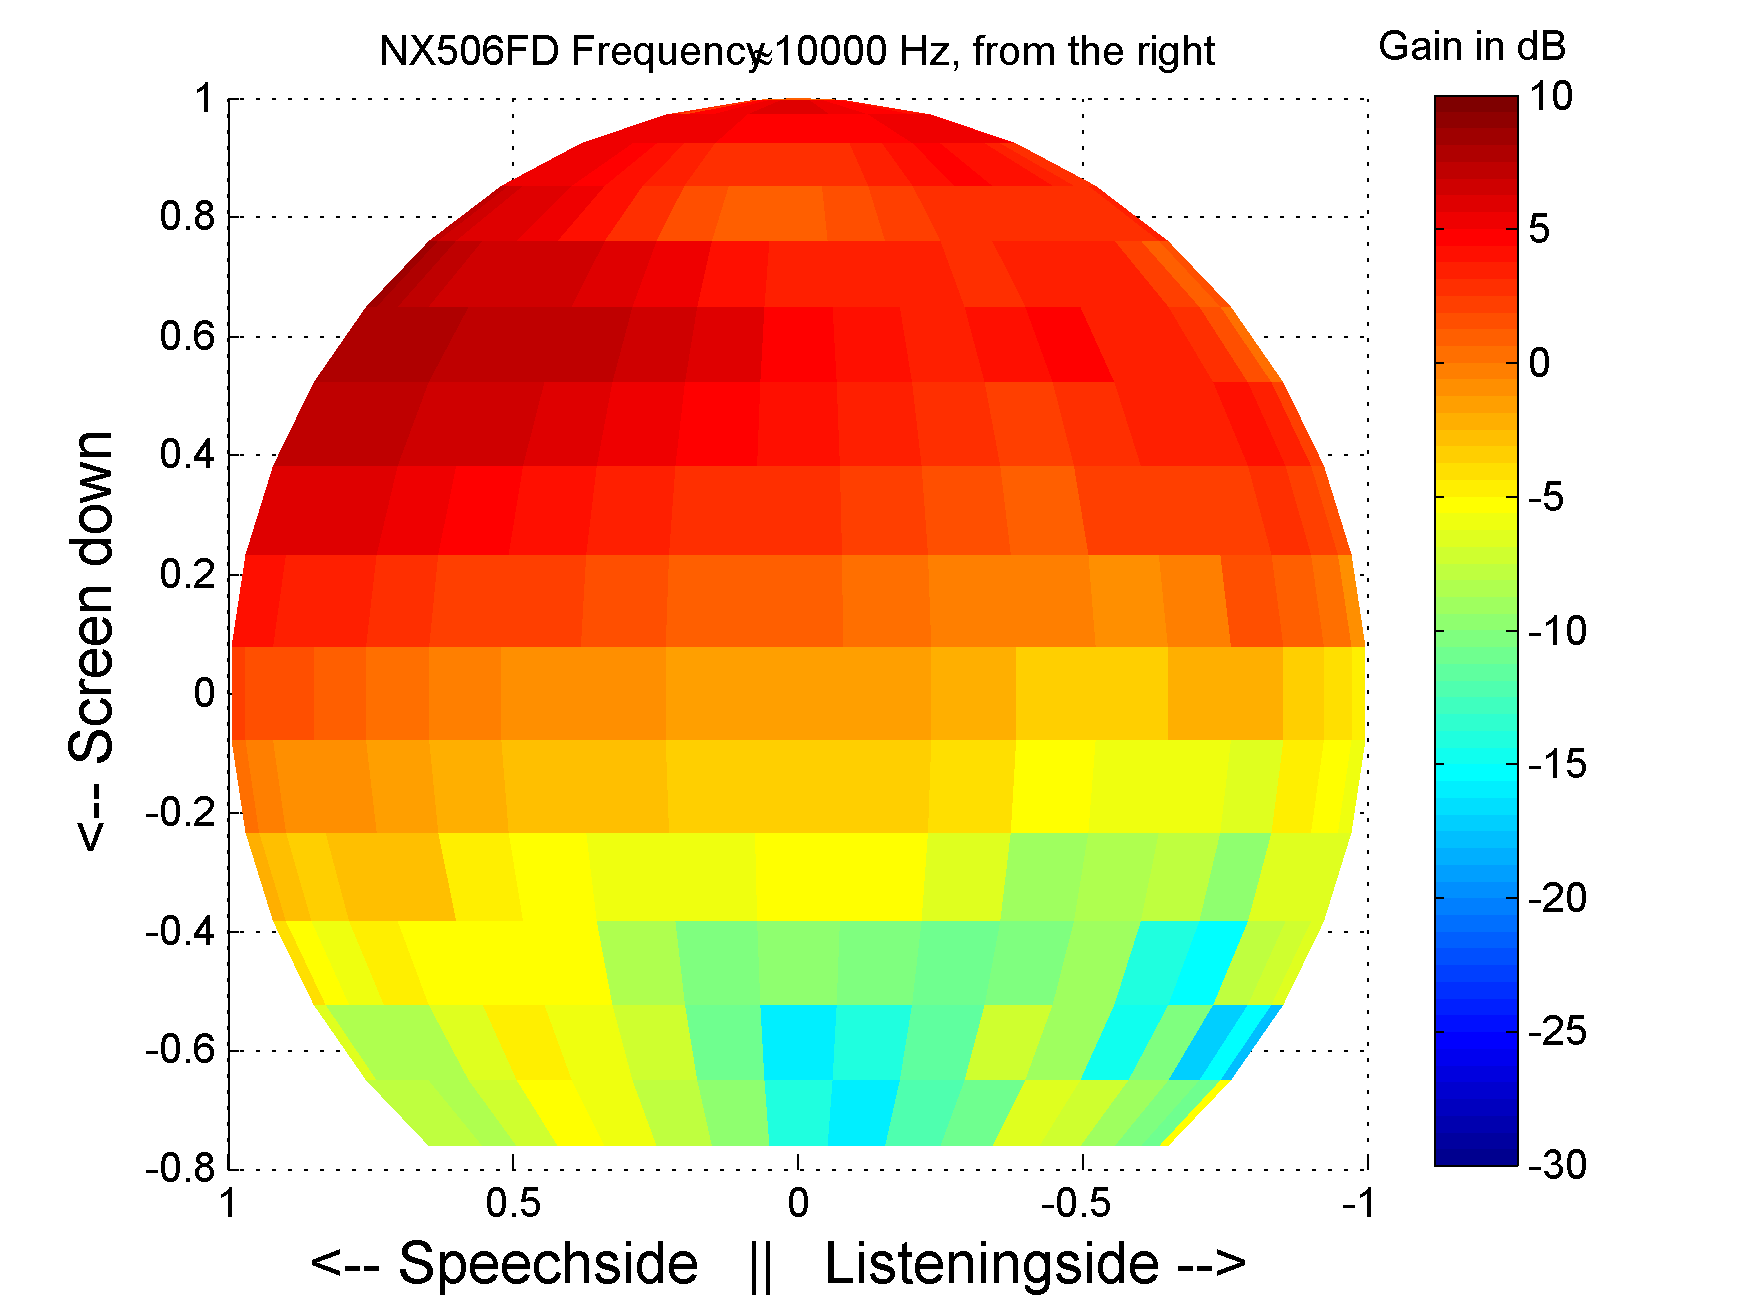
\includegraphics[height=0.28\textheight]{afbeeldingen/plots/results/NX506FD_10000_right.png}
        \end{subfigure}
\end{figure}

%%%%%%%%%%%%%%%%%%%%%%%%%%%%%%%%%%%%%%%%%%%%%%%%%%%%%%%%%%%%%%%%%%%%%%%%%%%%%%%%%%%%%%%%%%%%
% NX501 pluis
\clearpage
\begin{figure}[t!]
        \centering
        
        \caption[Measurement results {\nexus} (1), mid-air]{{\nexus}, labelled with number 1, measurements in mid-air, equalized}
        \label{fig:res_NX501_pluis}

        \begin{subfigure}[t]{0.5\textwidth}
			    \caption{$\phi=90^\circ$}
			    \label{fig:res_NX501_pluis_90}
                \centering
    			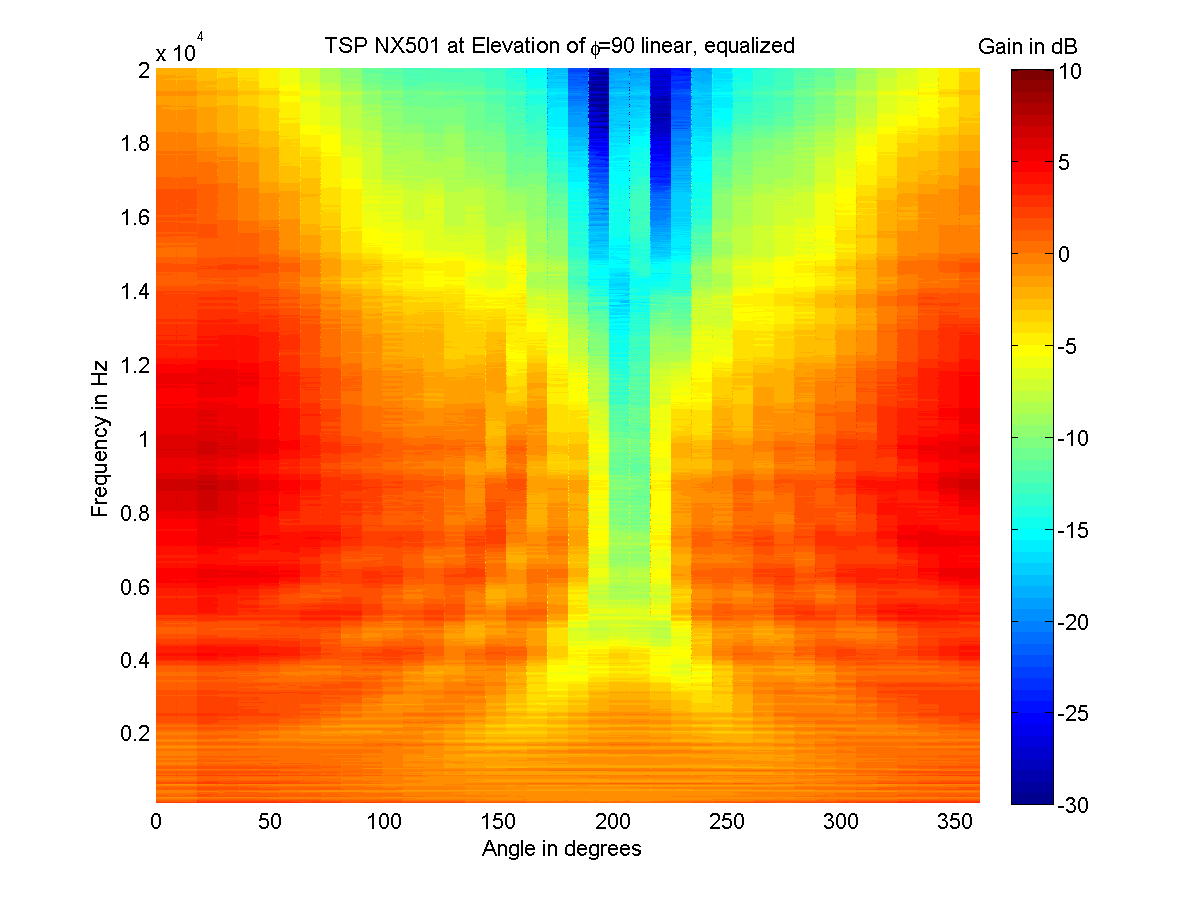
\includegraphics[height=0.28\textheight]{afbeeldingen/plots/results/NX501_TSP_090_lin_eq.png}
        \end{subfigure}~
        \begin{subfigure}[t]{0.5\textwidth}
			    \caption{$\phi=45^\circ$}
			    \label{fig:res_NX501_pluis_45}
                \centering
    			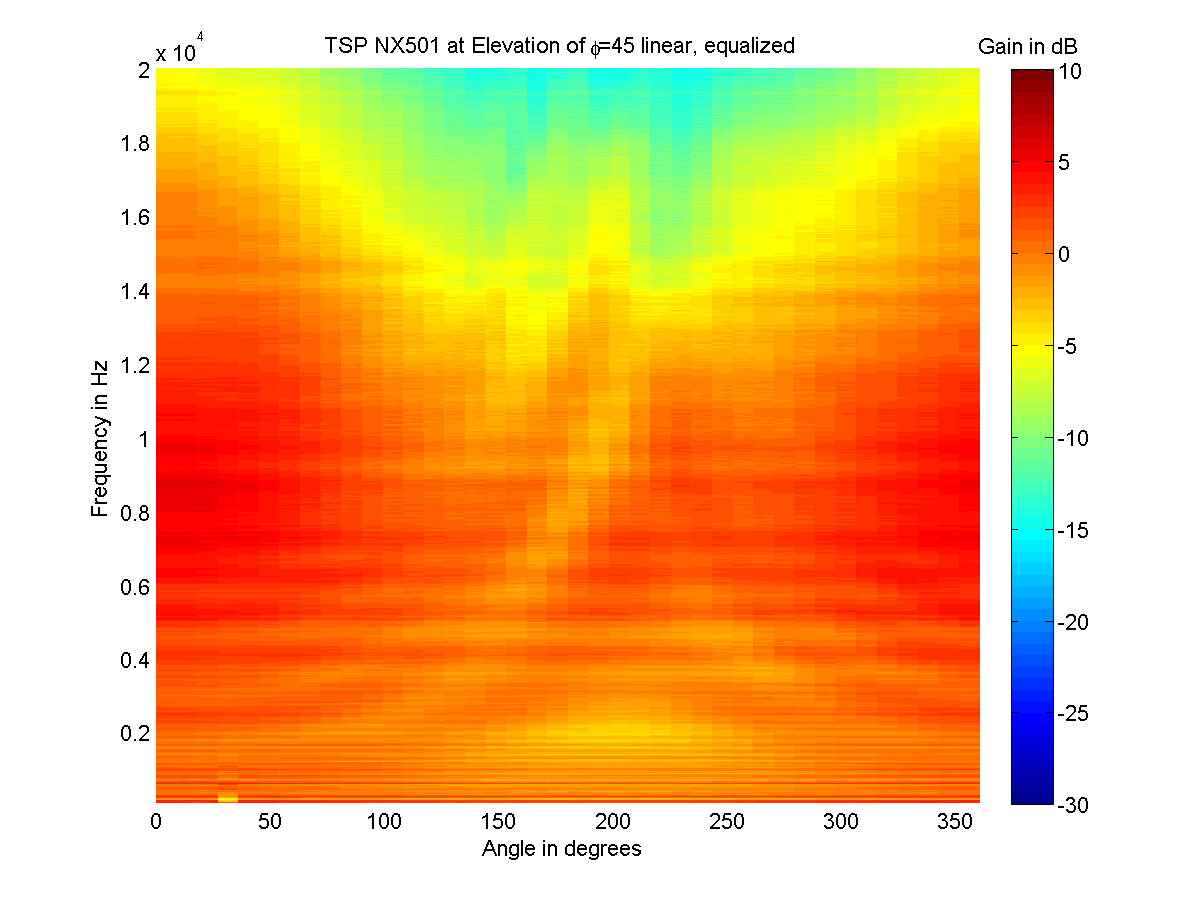
\includegraphics[height=0.28\textheight]{afbeeldingen/plots/results/NX501_TSP_045_lin_eq.png}
        \end{subfigure}
        
        \begin{subfigure}[t]{0.5\textwidth}
			    \caption{North pole: $\phi=0^\circ$}
			    \label{fig:res_NX501_pluis_0}
                \centering
    			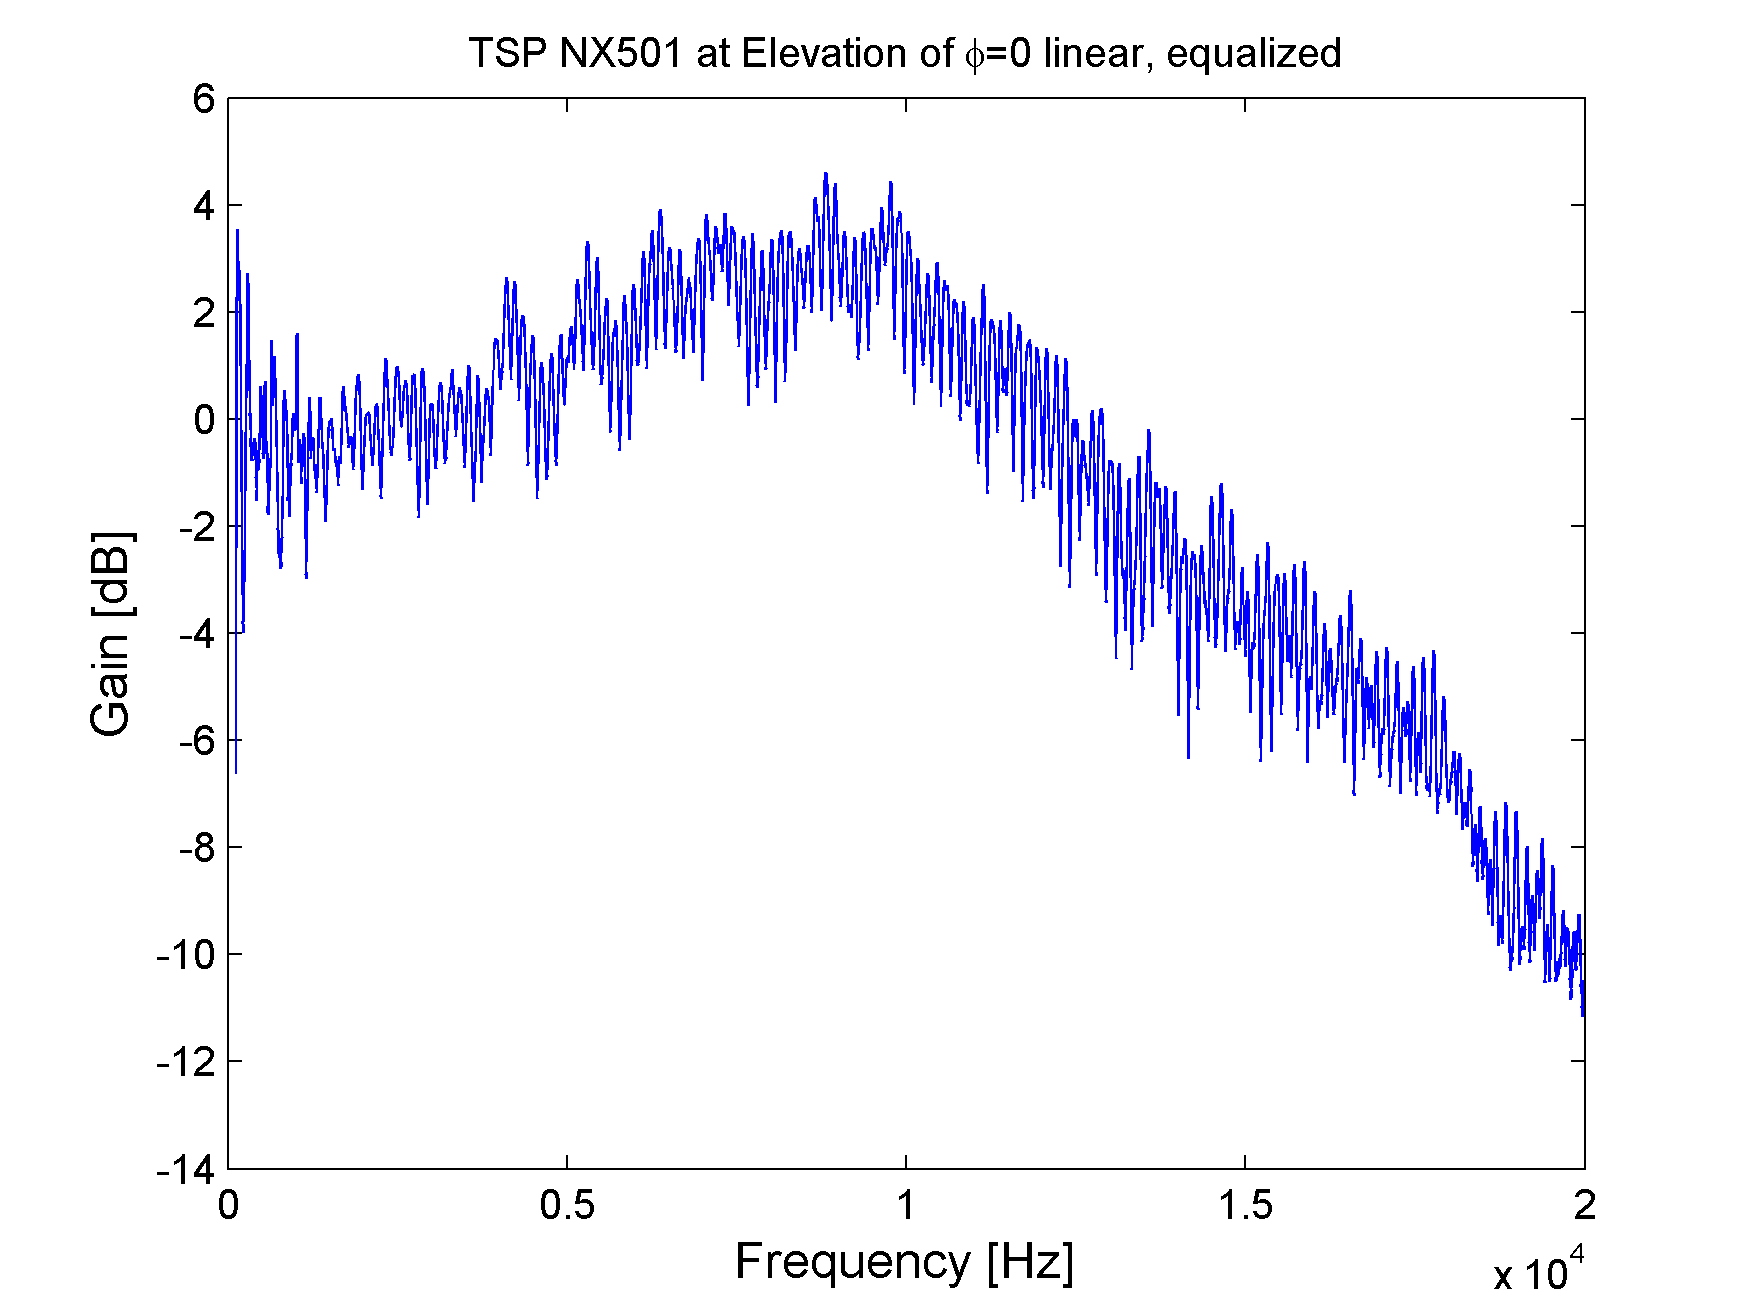
\includegraphics[height=0.28\textheight]{afbeeldingen/plots/results/NX501_north.png}
        \end{subfigure}
        
        \begin{subfigure}[t]{0.5\textwidth}
			    \caption{Upper half sphere $f=10000$ Hz, from the left}
			    \label{fig:res_NX501_pluis_sphere_left}
                \centering
    			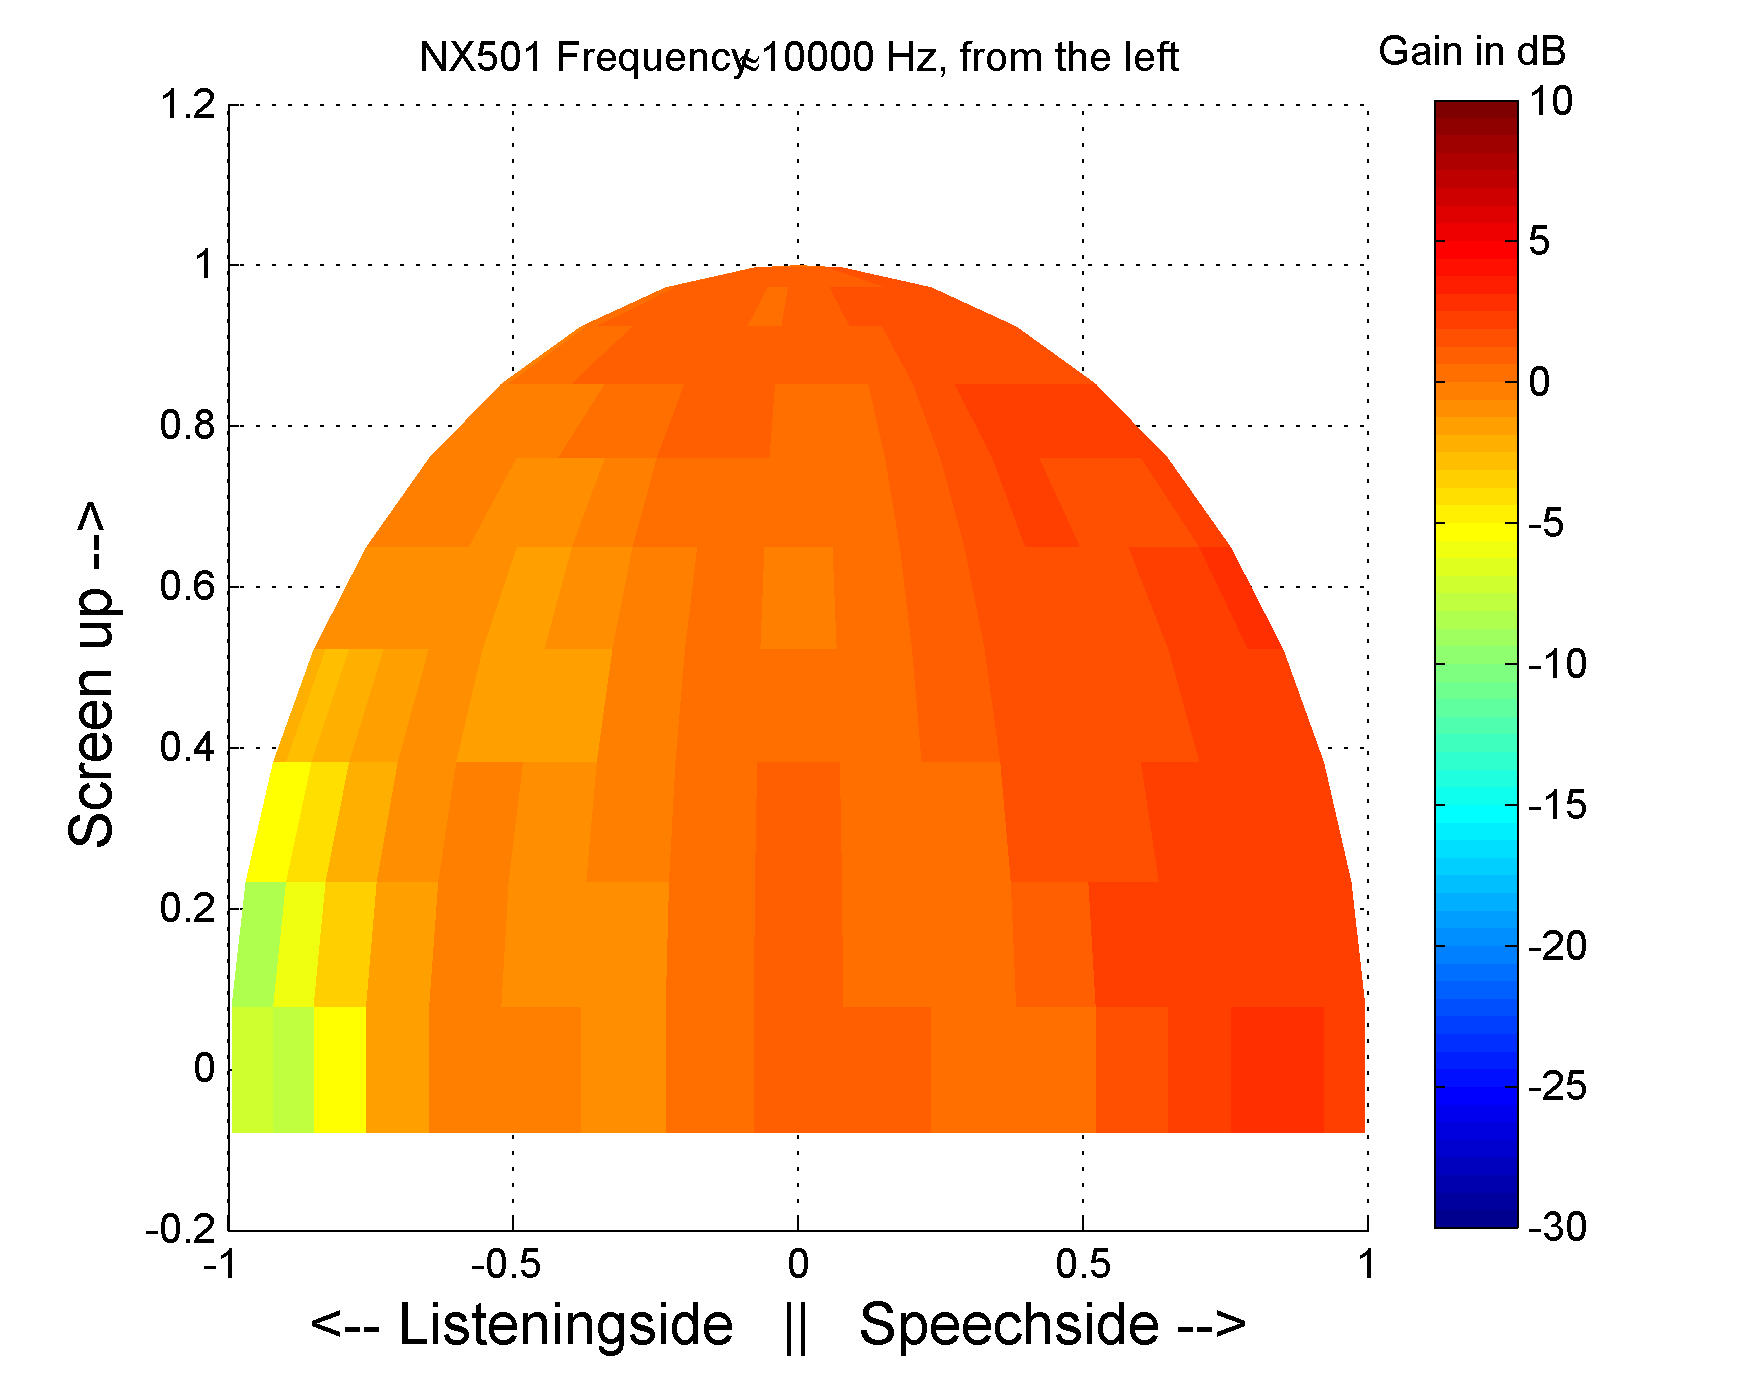
\includegraphics[height=0.28\textheight]{afbeeldingen/plots/results/NX501_10000_left.png}
        \end{subfigure}~
        \begin{subfigure}[t]{0.5\textwidth}
			    \caption{Upper half sphere $f=10000$ Hz, from the right}
			    \label{fig:res_NX501_pluis_sphere_right}
                \centering
    			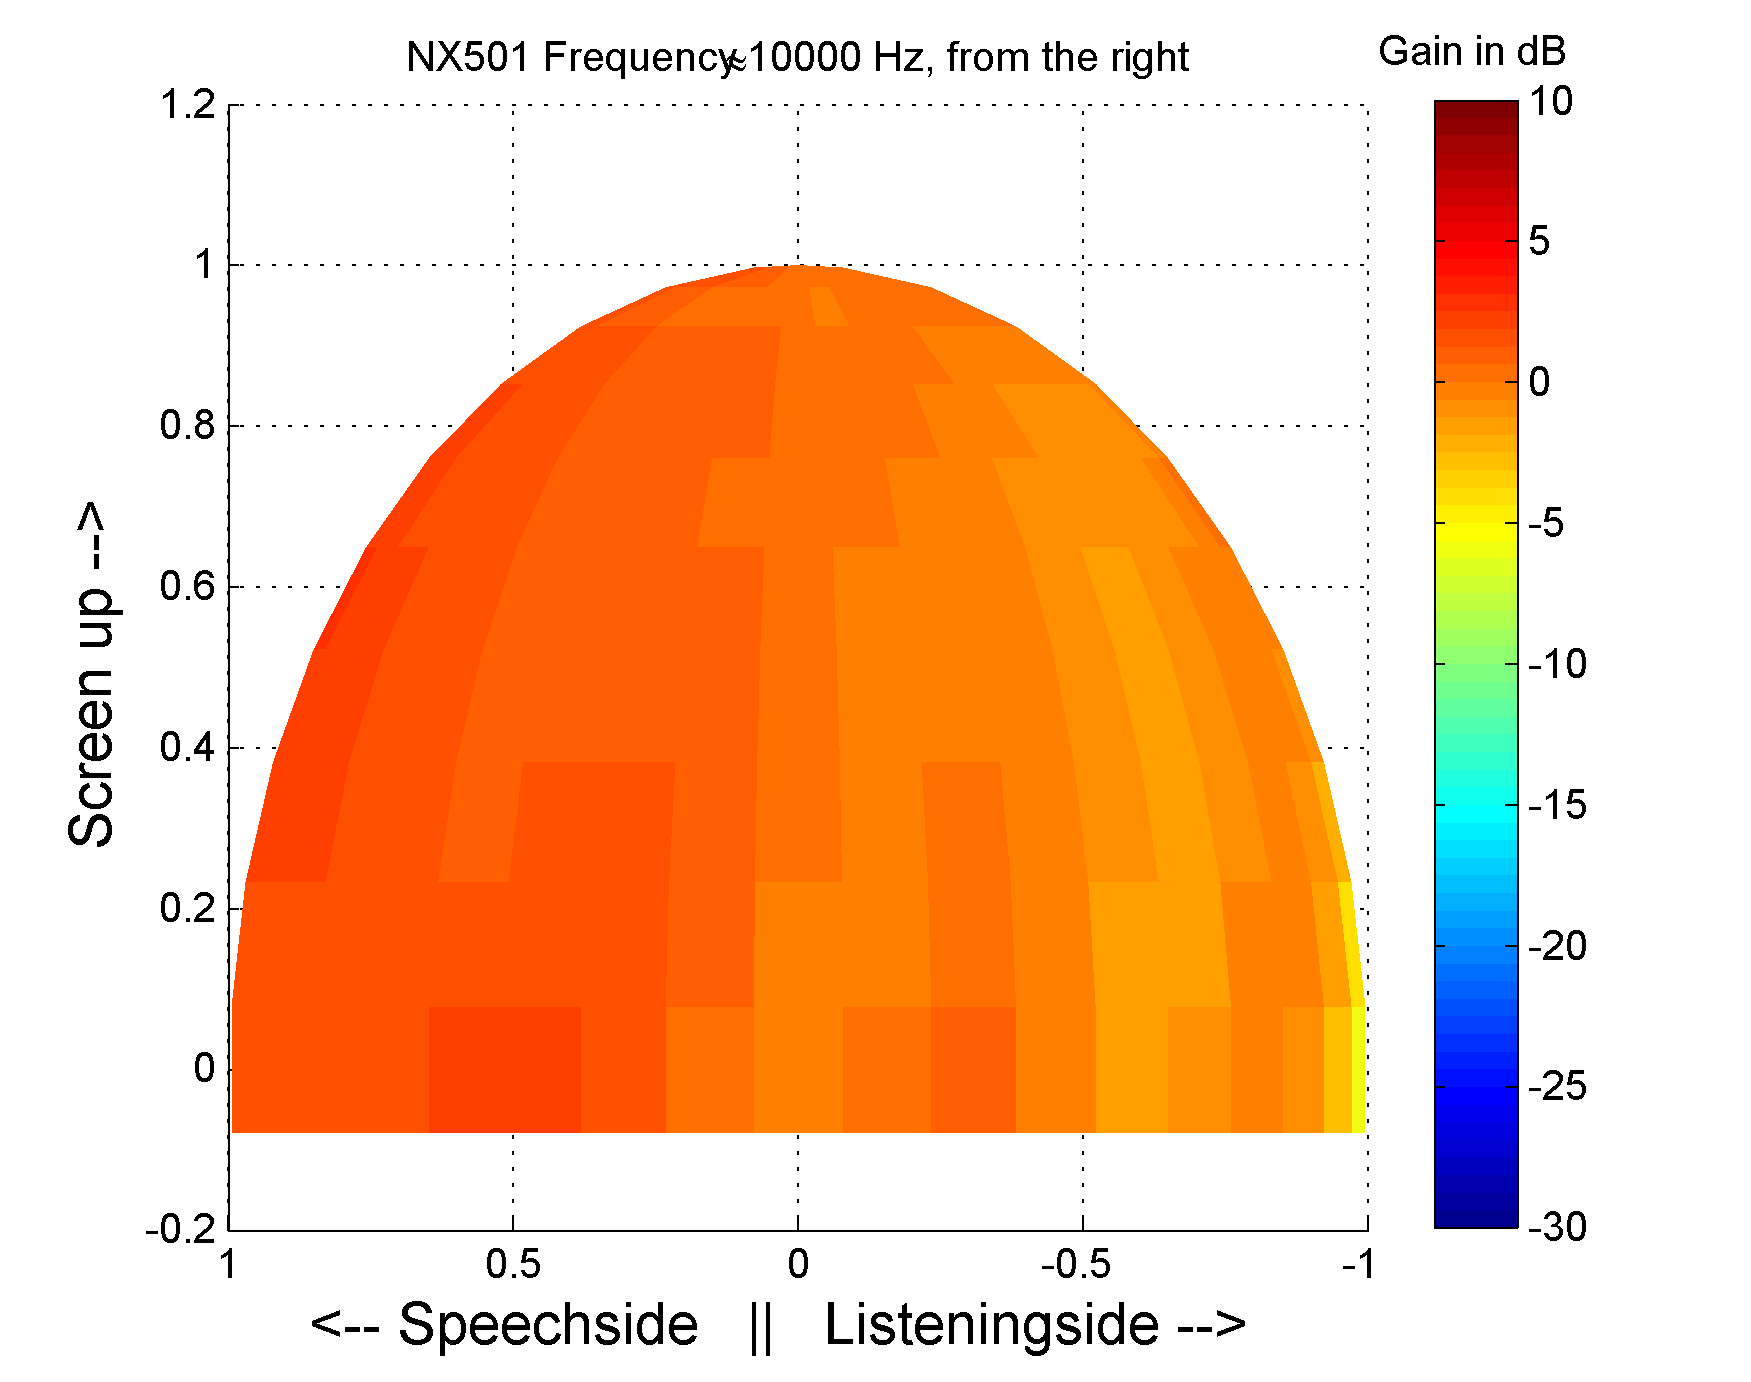
\includegraphics[height=0.28\textheight]{afbeeldingen/plots/results/NX501_10000_right.png}
        \end{subfigure}
\end{figure}